
\documentclass[a4paper]{article}

%opening

\title{\huge Functional Requirements And Software Architecture Specification
	\\COS 301 Team Alpha Project
	\\Version 2.0}

\author{\\\\Amy Lochner 14038600\\ Avinash Singh 14043778 \\
	Christiaan Nel 14029368\\ Christiaan Saaiman 12059138 \\
	Gerard van Wyk 14101263\\ Marc Antel 12026973\\
	Themba Mbhele 14007950
	\\
	\\
	\\\href{https://github.com/AvinashSingh786/COS301-Alpha.git}{GitHub}
	\textit{https://github.com/AvinashSingh786/COS301-Alpha.git}
	\\
	\\
	\\ University Of Pretoria\\}

\date{March 2016}

%\usepackage{graphicx}
\usepackage{float}
\usepackage{hyperref}
\usepackage{graphicx}
\usepackage{hyperref}
\hypersetup{
	colorlinks=true,
	linkcolor=blue,
	filecolor=magenta,      
	urlcolor=cyan,
}



\begin{document}
	
	\maketitle
	
	\pagenumbering{gobble}
	\newpage
	
	\tableofcontents
	\pagenumbering{arabic}
	\newpage
	
	\section{Introduction}
	
	This document defines the Software Requirements Specification and Technology Neutral Process Design for COS 301 Team Alpha. The Computer Science Department has expressed a need for the creation of a system, which can allow researchers to keep track of publications which they are currently working on, or have already published.
	\\
	The aim of this project is to follow a structured software development process in order to produce a product which provides the client with all the required functionality in an elegantly designed and built product. A collaborative and co-operative approach is required between all stakeholders who are involved in this project. 
	\\
	The information, specifications, and diagrams within this document are presented in order to provide testable requirements which correlate to the client's needs.
	
	\section{Vision}
	The client for this project, Ms. Vreda Pieterse who is a member of the Department of Computer Science at the University of Pretoria, has solicited us to develop a system. The purpose of this system is to record and oversee all publications of staff members or research groups, within the Department of Computer Science. The system will assist the Head of Department to track the progress on any papers which are in the process of being written; as well as determining whether or not a staff member is under performing thus allowing the Head of Department the opportunity to provide advice to these staff members.
	
	\section{Background}
	\subsection{The client's problem}
	The client has solicited us to develop a system that has specific usability goals, as well as certain user-experience goals. Currently, the Department of Computer Science does not have a system with which to monitor the progress of staff member's publications, nor to keep track of how many publications an author is working on. Furthermore, it is necessary to determine which publications will be presented at different conferences, as well as the reporting capabilities, and the ability to remind users of deadlines. The system should provide all these requirements in a secure, flexible and intuitive manner.
	
	
	\subsection{Future business/research opportunities}
	It is desired that this system will encourage authors to collaborate with other authors on similar topics and to expand the users base knowledge of ongoing research projects.
	\\
	\\
	\\
	
	% START OF ASSIGNMENT 2
	\section{Software Architecture Documentation ...}
	
	This document defines 
	
	\subsection{Architecture requirements}
	In this section extract the architectural requirements from the software requirements, including:
	
	\subsubsection{Architectural Scope}
	Architectural responsibilities that need to be addressed by the software architecture are as follows:
	\begin{itemize}
		\item Providing a persistent infrastructure - being a database stored on a dedicated server
		\item Providing a reporting infrastructure
		\item Providing an infrastructure for process execution
		\item Providing a backup infrastructure (e.g. making use of RAID)
		\item Providing a user interface through which the user can interact with the website/app
		\item Providing a means of Session management
		\item Providing a method of prevention against SQL injections
		\item Provide a log in system
		\item Provide a means with which to query the database in an interactive way
		\item Provide a means by which users can be notified about reminders
	\end{itemize}
	\subsubsection{Quality requirements}
	\begin{itemize}
		\item Performance \\\\
		The performance of a system refers to the behaviour of the system in terms of repsonse time and throughput. Changes and modifications to the system should be done in the most cost and time effective manner to provide a good user experience.
		One method of ensuring the performance is visible to the user is to make use of feedback tools to ensure the user is aware that the system is performing as expected or to notify the users should something have gone wrong.  
		\item Security \\\\
		Minimising the possibility of leaking information, maintaining data integrity, and avoiding session hijacking. This is very important as personal information will be stored in the database(e.g. email). The system will also have different user types with different access permissions hence security will be needed to ensure that a specific user only has the capabilities afforded to them. 
		\\\\
		We will achieve security by making use of 3 methods, namely: prevention, detection, and recovery.
		We will ensure that we have put means in place through which we may be able to detect any threats to the system, for example validating any information that is required to be sent to the server. Preventing threats to the system can be enforced through limiting the access channels, making use of authentication, not allowing any external sources to be accessed through the system, etc. Recovery will be achieved through cancelling requests and maintaining a working back up state to reroll changes.
		\item Maintainability \\\\
		This refers to how well the system can be modified to accommodate new functionality, access channels, fix bugs and improve the performance of the system. As it is likely that multiple people will be working on the system the code has to be easy to read and understand. We will achieve this by commenting our code to allow for a quick study of the code. We will employ a means by which to allow pluggability of our code to ensure that large amounts of code will not be needed to be changed/removed.
		\\\\
		The system should not only be maintainable in terms of issues with the system but it should also be maintainable in terms of usability, i.e user permissions should be allowed to be changed, etc.
		
		\item Scalability \\\\
		Scalabilty refers to the system's ability to handle increased traffic or workload. This will be implemented by ensuring that users can make the same requests simultaneously.
		\\\\
		We will need to ensure that resources are managed wisely in order to avoid lost updates, uncommitted data and inconsistent retrievals.
		
		\item Reliability \\\\
		As the system is required to support a fairly large user base it should allow for effective and safe concurrent use of the system. The system should ensure that no users can perform tasks that their user type does not afford to them.
		\\\\
		As access channels are via a web browser/android app it is essential that these access channels always have access to the server and thus database and ensure that the connection is stable, reliable and safe at all times. The system should be maintained in order to ensure that the system can perform all the required tasks in an effective and efficient manner. We will achieve this through unit testing, making use of concurrent resource locks and eliminating single points of failure.
		\item Auditability\\\\
		A requirement of the system is that all actions or changes to the should be logged to enable users with the appropriate permissions to be able to view all actions or changes to the system, who they were made by and when. This is essential in ensuring that the system can be rolled back to a stable state should something undesirable happen.
		\\\\
		We will implement this by having a log file running at all times which makes use of timestamping to indicate when changes were made, the system should allow to be rolled back to a stable state should it be deemed neccessary. ACID Properties will be applied to ensure that the database maintains a stable, reliable and current state.
		
		
		\item Integrability \\\\
		Will the system be able to integrate with other technologies.
		\item Usability \\\\
		Usability will be achieved through the implementation of an intuitive, easy to use, easy to understand and an aesthetically appealing interface through which the user will be able to perform all system functionality afforded to them through their user type.
		\\\\
		We will ensure that the user interface performs all tasks in the most efficient and direct means. The interface should not cause the user any irritation in the form of colour schemes, delayed functionality, over complication of tasks.
	\end{itemize}
	
	
	\subsection{Integration and access channel requirements}
	The CS Research System will serve as the basis of the entire system, possibly integrating with future systems. Integration can be made possible through the use of a RESTful API to enable cross-platform concurrent communication through HTTP or HTTPS. By using a service-oriented architecture and thereby componentizing the system, other systems can more easily integrate through service calls to these different components. A web interface as well as a mobile application, specifically on Android, should be made available for the end users. Other platforms should then be able to communicate with the system through simple REST API calls. Additionally, services such as Google Calendar and Google Mail can also be integrated into the system through simple API calls made available by Google. 
	\\
	
	\subsubsection{Architectural constraints}
	The architectural constraints as specified by the client include the following:
	\begin{itemize}
		\item Linux (Operating System, for the server)
		\item Android (Mobile Operating System, for the mobile application)
		\item HTTP (Hypertext Transfer Protocol, for cross-platform integration)
		\item HTML (Hypertext Markup Language for web client)
		\item PHP (Server Side Scripting, for personalised webpages)
		\item Java (Programming language, especially for the Android application)
		\item JavaScript (Programming language, for use in webpages)
	\end{itemize}
	\\
	
	\section{Architectural patterns or styles}
	Architectural Patterns are generally reusable solutions to commonly occuring problems within a given context. Similar to software design patterns, architectural patterns are 
	larger in scope though. The architectural patterns address various problems such as:
	\begin{itemize}
		\item Software Engineering
		\item Computer Hardware limitations
		\item High availablility
		\item Minimization of Business Risk
	\end{itemize}
	
	For this project and the scope thereof, I suggest either one of two architectures are used or possibly both.
	\subsection{Model-View-Controller}
	Model-View-Controller, here on out referred to as MVC, is popular architecture used for implementing systems with user-interfaces. Later this architecture
	became extremely popular for designing web applications and for this reason I suggest using this architecture. This architecture is easy to implement and 
	to maintain. It is divided into three seperate departments:
	\begin{itemize}
		\item The Model is in charge of managing the data, logic and rules of the system.
		\item The view is responsible for outputting the representation of the data that the user perceives.
		\item The controller takes in input and converts it to commands for the model & view.
	\end{itemize}
	Current day MVC architecture has moved away from thin client coding due to technologies such as AngularJS, EmberJS, JavaScriptMVC and Backbone.
	
	\subsection{Service-orientated Architecture}
	A service-oriented architecture (SOA) is an architectural pattern in computer software design in which application components provide services 
	to other components via a communications protocol, typically over a network. The principles of service-orientation are independent of any vendor, 
	product or technology.
	
	A service is a self-contained unit of functionality, such as retrieving an online bank statement. By that definition, a service is an operation
	that may be discretely invoked. However, in the Web Services Description Language (WSDL), a service is an interface definition that may list several
	discrete services/operations. And elsewhere, the term service is used for a component that is encapsulated behind an interface. This widespread
	ambiguity is reflected in what follows.
	
	Services can be combined to provide the functionality of a large software application. SOA makes it easier for software components on computers
	connected over a network to cooperate. Every computer can run any number of services, and each service is built in a way that ensures that the service
	can exchange information with any other service in the network without human interaction and without the need to make changes to the underlying program
	itself.
	
	
	\section{Architectural tactics or strategies}
	In this section, we will discuss certain strategies that will be used to achieve the quality requirements stated in section 4.1.2.
	\begin{itemize}
		\item Hashing and Salting Passwords \\\\
		To ensure that sensitive information of the users of the system is not leaked in the event of a database compromise, all passwords will not be stored in plain text. Instead, all passwords will be hashed with a strong one-way hashing algorithm, such as the sha256, so that in the event of a database compromise, it will be near impossible to compute the actual passwords from the hashes. To make the hashes more effective, we will add random data, known as salt, to the passwords before hashing them. This will make it extremely difficult for intruders to use pre-hashed tables to perform a look up to find a matching password.
		\\
		\item Prepared Statements \\\\
		To prevent the illegal extraction of data and/or the destruction of data from the database through SQL injection and blind SQL injection attacks, we will make use of prepared statements. Prepared statements also have other benefits other than security. Even though prepared statements execute a statement multiple time, they reduce parsing time as the preparation of the query is only done once. This will improve the efficiency and performance of the system. Also, because prepared statements bind values to parameters, the bandwidth on the server is minimized because you only need to send the parameters to the server and not the whole query. This also improves the performance of the system.
		\\
		\item Caching \\\\
		Because the system relies heavenly on databases, there will be a significant number of access attempts to the the databases. This has the potential of creating a bottleneck that gets worse as the number of concurrent users increases. This means that the system will scale poorly and the performance of the system will decrease drastically. The best way to combat this is to limit accesses to the databases were possible. To accomplish this, we will make use of a distributed cache system. A distributed cache will particularly be effective in read operations and will provide large performance gains as it reduces the processing times of applications and it limits database accesses. This will improve the scalability of the system drastically and thus will accommodate a large number of concurrent users. 
		\\
		\item Database Normalization \\\\
		To make the system flexible, we will create the database tables and link them to one another were it is appropriate to do so according to rules that protect the data and makes it flexible. This process is known as normalization. Normalization eliminates redundancies and inconsistent dependencies. This makes it simple to makes changes to the system and also makes it easy to add new components to the system.
		\\
	\end{itemize}
	\section{Use of reference architectures and frameworks ...}
	...\\ 
	\section{Access and integration channels}
	%Avinash Singh
	\subsubsection{Apache CouchDB Database System}
	Apache CouchDB, the database commonly referred to CouchDB is a document-oriented NoSQL database that is open source. Integration with this system is required for retrieval of the majority of the information that the system will require. Performance for this channel is also crucial since we need fast and superior access speeds since the system mostly relies on querying with the database and thus this system has implemented MVCC - Multi Version Concurrency Control so it can process multiple queries with good response time. Furthermore this database makes use of JSON - JavaScript Object Notation, which transfers encrypted objects and is more dense and more faster than XML - Extensible Markup Language
	
	\paragraph{Quality Requirements for the Database System}
	\begin{itemize}
		\item{\textbf{Performance:} All queries to the CouchDB database should be rapid and efficient to provide the best user experience to the maximum amount of people. This is achieved through the MVCC since it can perform multiple queries at once as well as it makes use of JSON, which on its own is fast.}
		\item{\textbf{Reliability:} It is important that the system needs to have as some downtime for upgrading and maintaining, thus a reliable connection to the Couchbase server is needed. }
		\item{\textbf{Scalability:} The system needs to be able to work with a large amount of users concurrently. This is met with the MVCC and thus the Couchbase Server is the best suited.}
		\item{\textbf{Integrability:} The integration with the CouchDB database should be engineered in a manner which can easily be adjusted to accommodate additional integrations. Since this is a Web based system and CouchDB is built for Web since it uses HTTP protocol and JavaScript querying.}
		\item{\textbf{Affordability:} Access or queries made to the CouchDB database should be affordable, this is met since CouchDB is open source there is no physical money involved and requests made as often as needed are done without any implications, and does not affect the overall system performance.}
		\item{\textbf{Flexibility:} The integration with the database should be flexible in the sense that slight changes in the database functionality should not affect the integration with the System. This is met since the database has a merging algorithm and manages conflicts on its own.}
		\item{\textbf{Auditability:} Any modifications made, user interactions, queries should be announced. This can be done through Identification, time-stamps, digital receipts and this should be linked to the integration channels used. Every integration action must be traceable to a user or system action to provide debugging and easy maintenance.}
	\end{itemize}
	
	
	
	
	\subsubsection{Web services}
	Web services to be used namely HTTP, HTTPS and TCP, will facilitate user interaction with the system. and provide security to the system. 
	\paragraph{Quality Requirements for the Web Services}
	\begin{itemize}
		\item{\textbf{Security:} This is a very important requirement since in any web-based application needs to be secure if it involves sessions and logging into the system, it must incorporate user authentication and the storage of personal information as well as a digital certificate to make sure that the connection is secure.}
		\item{\textbf{Reliability:} For this it should be minimalist downtime, since there will be a lot of users and that need the services of the system so it should still have some interaction when down. }
		\item{\textbf{Integrability:} Web services need to be integrated with a host of other services like Google or any other future organizations that add more functionality and features to the system, typically notification system where the user can get notifications via different methods or services.}
		\item{\textbf{Performance:} This is a major priority to avoid lowering the overall system performance, since there are a vast range of web services available this must be achieved. However the use of a secured connection can tend to have some performance decrease since there is a lot more to process and is a bit slower than HTTP, but the increased security always is better over performace there us no use if the system is fast but has a security flaw.}
		\item{\textbf{Scalability:} The protocols utilized need to be able to cope with all the concurrent users connected to the system without breaking down or crashing down and perform optimally.}
	\end{itemize}
	
	\subsection{Access channels}
	The system has various access channels from which users can gain access to the system:
	\begin{itemize}
		\item Computer - All users of the system should be able to access the system through the Internet/browser. Users will can use a modern web browser, such as Mozilla Firefox, Google Chrome, Microsoft Internet Explorer, or Apple Safari to interact with the system. All users will be required to login to the system to make use of the features available.
		\item Mobile - Users will also have access to system via an Android application, as well as the web application should have support for the mobile devices.
	\end{itemize} 	
	
	
	\subsection{Protocols}
	\subsubsection{Database Query Language}
	JavaScript will be used to query the CouchDB database by making use of MapReduce.
	
	\subsubsection{HTTP - Hypertext Transfer Protocol}
	Integration with this protocol will deal with links and to exchange or transfer hypertext at typically handled by the web browser or certain libraries, HTTP is commonly found in RFC 2068 in 1997. HTTP is situated in the application layer of the network stack so it is high level.
	\textbf{Used for:	}
	\begin{itemize}
		\item{Handling all the socket communications between the client and server, this entails all the data transfer.}
		\item{Data transfer between the system and database either using TCP or UDP.}
		\item{Transfer of log data such as error codes to ensure both servers and clients are aware of the state of data transfers and its results}
	\end{itemize}
	
	
	\subsubsection{HTTPS - Hypertext Transfer Protocol Secure}
	The same as HTTP only that this is secured and uses SSL - Secure Socket Layer, which has encryption added to the Transport layer. 
	\textbf{Used for:	}
	\begin{itemize}
		\item{Handling all the socket communications between the client and server in a secure fashion using certificates and keys.}
		\item{Preventing eavesdropping and tampering, so that hackers can't steal or access your personal information and to make the user sure that the browser is connected to the server directly so that there is no middle man.}
		\item{Transfer of log data such as error codes to ensure both servers and clients are aware of the state of data transfers and its results.}
	\end{itemize}
	\subsubsection{TCP - Transmission Control Protocol}
	This protocol is the core protocol of the Internet protocol  suite, it is reliable, ordered and has error-checking stream between applications running on hosts over the network
	\textbf{Used for:	}
	\begin{itemize}
		\item{It detects faults and monitors traffic with load balancing, some packets can get lost this protocol sees if it does and requests retransmission of lost data.}
	\end{itemize}
	\subsubsection{SMTP - Simple Mail Transfer Protocol}
	This protocol is an standard for mail transfer over the net that uses RFC 5321, which is a widespread protocol that uses the default port 25
	\textbf{Used for:	}
	\begin{itemize}
		\item{Manage e-mail communication in the system, being able to send the notifications to the users when a publication is due for submitting.}
		\item{Required to be able to send concurrent e-mails as well as in a hierarchical structure.}
		\item{Sending secure e-mails to the users without having any malicious code injected.}
	\end{itemize}
	
	\subsection{API specifications}
	\subsubsection{Apache CouchDB}
	Makes use of JavaScript querying using MapReduce and uses the HTTP API
	
	\subsection{JavaScript}
	This is a very functional web framework that has a wide variety of functions and plug-ins, also a vast variety of other frameworks that integrate into it. It has its own API for text, arrays and regular expressions
	\subsubsection{GIT}
	GIT can be used as a version control API as it will allow an easy means to manage the versions and also solve code conflicts and allow multiple programmers to collaborate and code together.
	
	\subsubsection{REST -Representational state transfer}
	Paves the software architecture of the World Wide Web
	\textbf{Architecture properties}
	\begin{itemize}
		\item{Performance - efficient and has dominating component interactions.}
		\item{Scalability - supports a large amount of components.}
		\item{Simplicity - makes use of interfaces.}
		\item{Modifiability - components can be changed or modified even during run-time.)
			\item{Visibility - communication between components by the different service agents.}
			\item{Portability, - code can be moved with the data through the components.}
			\item{Reliability - has methods with dealing for failures.}
		\end{itemize}
		
		

	
	
	%
	\section{Technologies}
	The following technologies will be used to develop the Research System:
	\begin{itemize}
		\item HTML (Hypertext Markup Language): A standardized system for tagging text files to achieve font, colour, graphic, and hyperlink effects on World Wide Web pages. This will be the interface for the users of the system. 
		\item AJAX (Asynchronous JavaScript and XML): Ajax is a group of interrelated Web development techniques used on the client-side to create asynchronous Web applications. The use of Ajax will bring dynamic changes to the web page. This will update changes to the system without the user having to refresh the page and will avoid identical information being submitted multiple times by multiple users. 
		\item JavaEE (Java Platform Enterprise Edition): This platform provides an API and runtime environment for developing and running enterprise software, including network and web services, and other large-scale, multi-tiered, scalable, reliable, and secure network applications. JavaEE is fundamental for the Research System in providing the connections for the user to the system.
		\item JavaScript (Functionality to HTML): An object-oriented computer programming language commonly used to create interactive effects within web browsers. This will enhance the functionality and appearance of the web pages of the Research System.
		\item PHP (Server Side Scripting): PHP is a server scripting language, and a powerful tool for making dynamic and interactive Web pages. The Research System will use PHP for collecting data from forms, such as adding a user and adding a publication. 
		\item MySQL (Database Manager): MySQL is a database system used on the web, which runs on the server. This will be the chosen database system, since it is very fast, reliable, and easy to use, as well as being able to compile on a number of platforms.
		\item Android (Mobile Devices): Android is a mobile operating system, which is designed primarily for touchscreen mobile devices such as smartphones and tablets. An android application will be developed for the Research System, to provide an easy to use interface for the user on mobile devices.
		\item Apache (Web Server): The Apache HTTP Server is the world's most used web server software. This is the chosen its performance and reliability, as well as being able to support the other technologies that the Research System will be using. 
		\item Linux/Windows/Mac (Operating System): The three operating systems that are most commonly used today. The Research System will have to be able to run in these three Operating Systems.
		\\
		\\
	\end{itemize}
	\pagebreak
	
	
	
	%END
	
	
	
	
	
	
	
	
	
	
	
	
	
	
	
	
	\section{Functional Requirements and Application Design}
	This section discusses the application functionality and service contracts required by the users.
	\subsection{Use Case Prioritization}
	The Use Case Prioritisation is specified for each use case in the next section.
	
	\subsection{Use Case/Services Contracts}
	Use Case Prioritisation and Service Contracts are described below
	
	\subsubsection{User Login}
	\textbf{Description:}  A user is required to log into the system before the user can make use of any functionality.
	\\
	\textbf{Prioritisation:} Critical\\
	
	
	\textbf{Pre-conditions}
	\begin{itemize}
		\item A user must have a connection to the server.
		\item A user must be registered as a user by a person with HOD or Admin permission.
		\item The user must enter the correct information in order for the authentication to be successful.
	\end{itemize}
	
	\textbf{Post-conditions}
	\begin{itemize}
		\item The user has specific access to the server on which all data is stored, i.e add/edit authors and search for authors
		\item The user is able to use all the user functionality provided by the system 
		\item The user may log out of the system when they wish to.
	\end{itemize}
	
	\begin{figure}[H]
		\centering
		%            		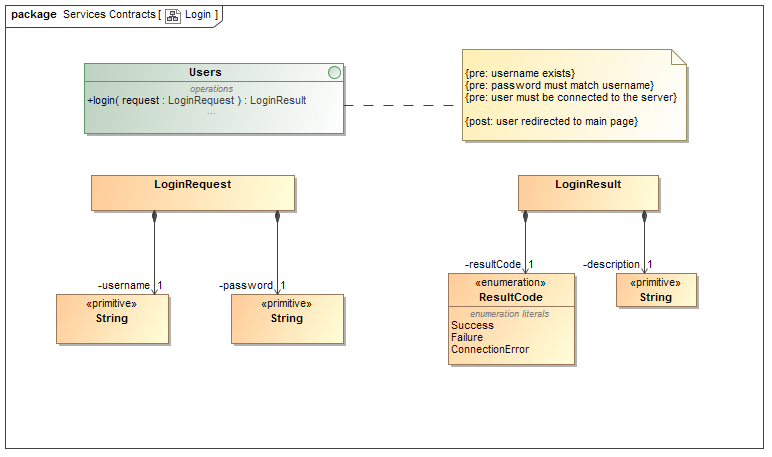
\includegraphics[width=\textwidth]{../Assignment1/5.1.1.Login.Services.Contract.png}
		\caption{Service Contract: User Login}
	\end{figure}
	
	\pagebreak
	\subsubsection{User Registration}
	
	\textbf{Description:}  In order to be able to log into the system and make use of the functionality provided by the system the user must be registered on the system. \\
	\textbf{Prioritisation:} Critical\\
	
	\textbf{Pre-conditions}
	\begin{itemize}
		\item The user must be part of the staff of the Computer Science Department of the University of Pretoria.
		\item The administrator or HOD of the system must have registered the user on the system.
		\item The user must decide on their login credentials.
	\end{itemize}
	
	\textbf{Post-conditions}
	\begin{itemize}
		\item The user's login information is securely stored in the system database.
		\item The user can log into the system.
	\end{itemize}
	
	\begin{figure}[H]
		\centering
		%        		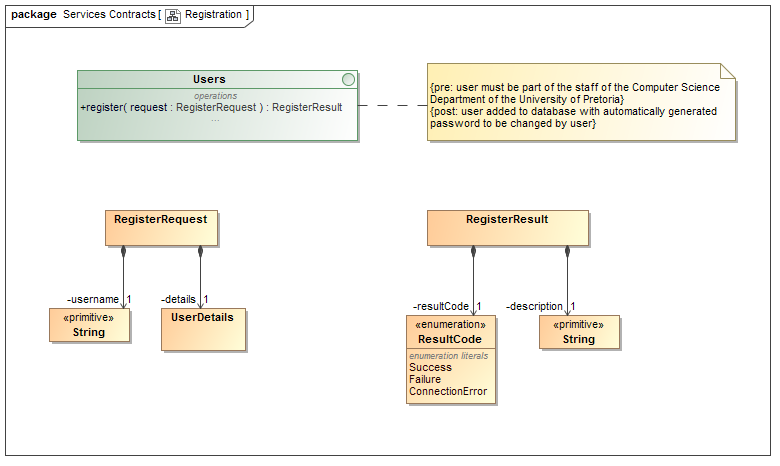
\includegraphics[width=\textwidth]{../Assignment1/5.1.2.Registration.Services.Contract.png}
		\caption{Service Contract: User Registration}
	\end{figure}
	
	
	\pagebreak
	\subsubsection{Update User}
	
	\textbf{Description:} Personal details as well as log in credentials can be changed if and when necessary.\\
	\textbf{Prioritisation:} Important\\
	
	\textbf{Pre-conditions}
	\begin{itemize}
		\item The administrator or HOD must be logged into the system.
		\item The user to be updated must already exist in the system.
		\item The administrator or HOD must have the new information.
	\end{itemize}
	
	\textbf{Post-conditions}
	\begin{itemize}
		\item The user's information is updated on the system's database.
	\end{itemize}
	
	\begin{figure}[H]
		\centering
		%            		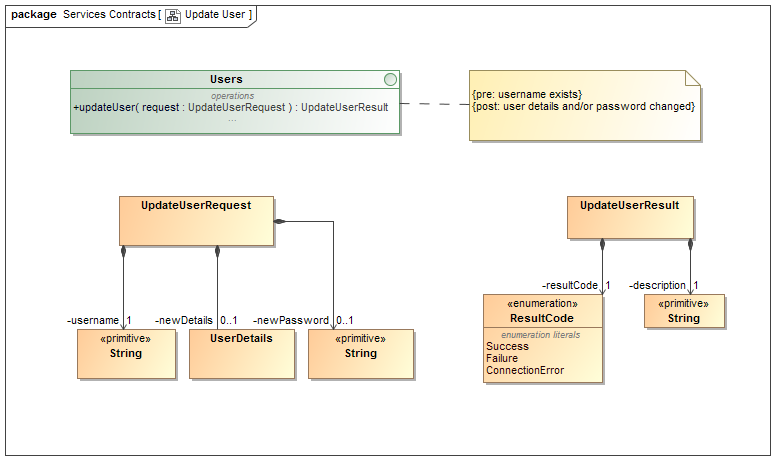
\includegraphics[width=\textwidth]{../Assignment1/5.1.3.Update.User.Services.Contract.png}
		\caption{Service Contract: Update User}
	\end{figure}
	\pagebreak
	\subsubsection{Remove User}
	
	\textbf{Description:} Should a user no longer belong to the Department of Computer Science the person should be removed from the system.\\
	\textbf{Prioritisation:} Important\\
	
	\textbf{Pre-conditions}
	\begin{itemize}
		\item The person should be a user on the system.
		\item The person should no longer belong to the staff of the Department of Computer Science.
		\item The administrator or HOD must be the logged in.
	\end{itemize}
	
	\textbf{Post-conditions}
	\begin{itemize}
		\item The person is removed from the system's database.
		\item The person can no longer gain access to the system.
		\item The person history still remains in the log file.
	\end{itemize}
	
	\begin{figure}[H]
		\centering
		%        		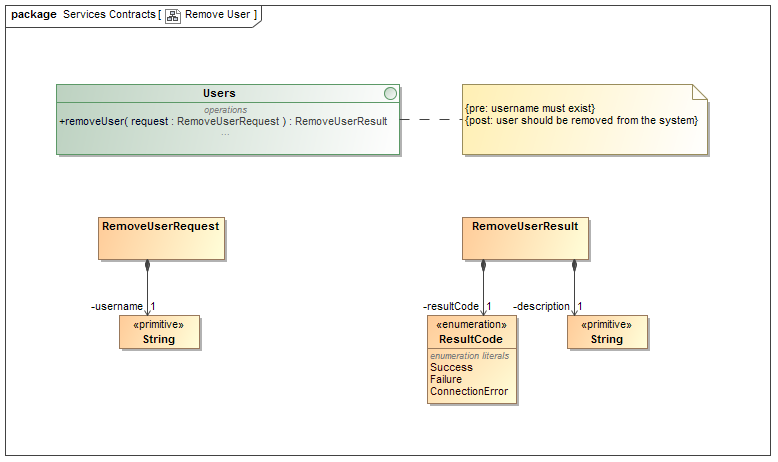
\includegraphics[width=\textwidth]{../Assignment1/5.1.4.Remove.User.Services.Contract.png}
		\caption{Service Contract: Remove User}
	\end{figure}
	\pagebreak
	\subsubsection{Create Publication}
	
	\textbf{Description:} Adding a paper to the system\\
	\textbf{Prioritisation:} Critical\\
	
	
	\textbf{Pre-conditions}
	\begin{itemize}
		\item The user(may be the administrator or HOD) should be logged into the system.
		\item The user, if not the administrator or HOD, must be a contributor to the paper.
		\item All authors who contributed to the paper should be available on the system.
	\end{itemize}
	
	\textbf{Post-conditions}
	\begin{itemize}
		\item The paper is added to the system
	\end{itemize}
	
	\begin{figure}[H]
		\centering
		%            		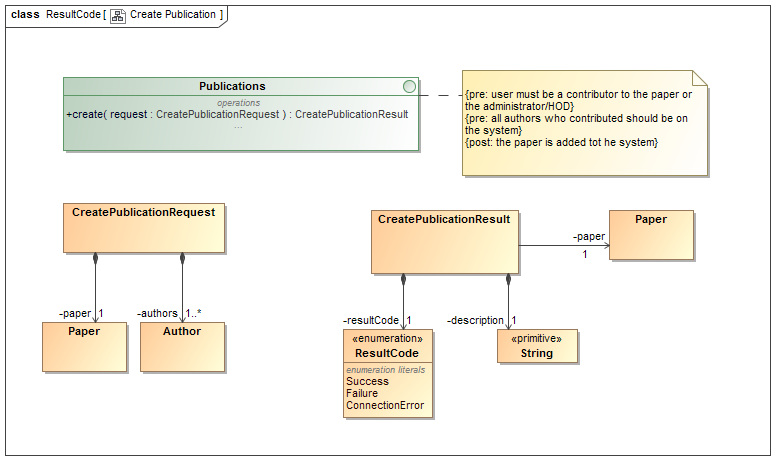
\includegraphics[width=\textwidth]{../Assignment1/5.1.5.Create.Publication.Services.Contract.png}
		\caption{Service Contract: Create Publication}
	\end{figure}
	\pagebreak
	\subsubsection{Update Publication}
	
	\textbf{Description:} Allows a user/administrator/HOD to change a publication's meta-data\\
	\textbf{Prioritisation:} Critical\\
	\\
	
	\textbf{Pre-conditions}
	\begin{itemize}
		\item The user(may be the administrator or HOD) should be logged into the system.
		\item The user, if not the administrator or HOD, must be a contributor to the paper.
		\item The paper must already be in the system.
	\end{itemize}
	
	\textbf{Post-conditions}
	\begin{itemize}
		\item The paper's meta-data is updated
	\end{itemize}
	
	\begin{figure}[H]
		\centering
		%            		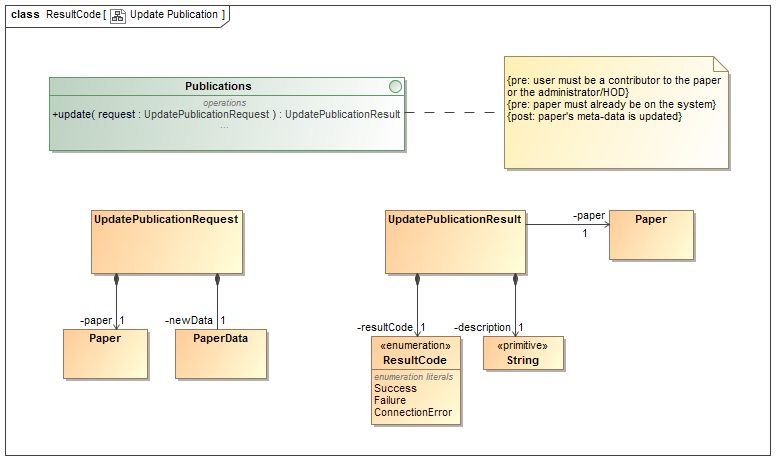
\includegraphics[width=\textwidth]{../Assignment1/5.1.6.Update.Publication.Services.Contract.png}
		\caption{Service Contract: Update Publication}
	\end{figure}
	\pagebreak
	\subsubsection{View Publication}
	
	\textbf{Description:} Allows a user/administrator/HOD to view the meta-data of a paper that lies within their permissions\\
	\textbf{Prioritisation:} Important\\
	\\
	
	\textbf{Pre-conditions}
	\begin{itemize}
		\item The user(may be the administrator or HOD) should be logged into the system.
		\item The user - if not the administrator, HOD or research leader - must be a contributor to the paper.
		\item The paper must already be in the system.
	\end{itemize}
	
	\textbf{Post-conditions}
	\begin{itemize}
		\item The paper's meta-data is displayed to the user
	\end{itemize}
	
	\begin{figure}[H]
		\centering
		%                		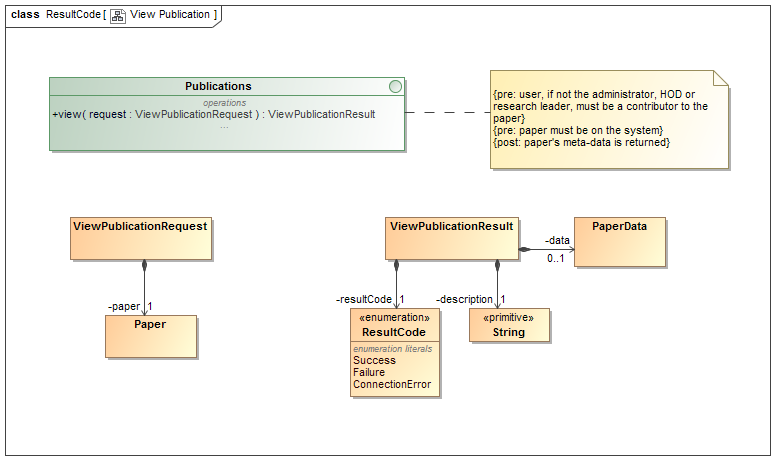
\includegraphics[width=\textwidth]{../Assignment1/5.1.7.View.Publication.Services.Contract.png}
		\caption{Service Contract: View Publication}
	\end{figure}
	
	\pagebreak
	\subsubsection{Add Publication Type}
	
	\textbf{Description:} Allows the administrator or HOD to add a publication type \\
	\textbf{Prioritisation:} Important\\
	\\
	
	
	\textbf{Pre-conditions}
	\begin{itemize}
		\item The user(must be the administrator or HOD) should be logged into the system.
		\item The publication type to add must not already be in the system.
	\end{itemize}
	
	\textbf{Post-conditions}
	\begin{itemize}
		\item The new publication type is added to the system.
	\end{itemize}
	
	
	\begin{figure}[H]
		\centering
		%            	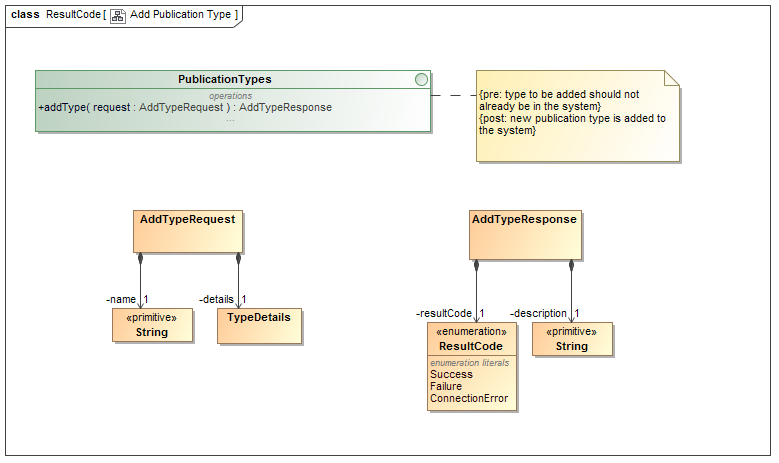
\includegraphics[width=\textwidth]{../Assignment1/5.1.8.Add.Publication.Type.Services.Contract.png}
		\caption{Service Contract: Add Publication}
	\end{figure}
	
	\pagebreak
	\subsubsection{Update Publication Type}
	
	\textbf{Description:} Allows the administrator or HOD to update a publication type's details\\
	\textbf{Prioritisation:} Important\\
	
	
	\textbf{Pre-conditions}
	\begin{itemize}
		\item The user(must be the administrator or HOD) should be logged into the system.
		\item The user - if not the administrator, HOD or research leader - must be a contributor to the paper.
		\item The publication type to be updated must already be in the system.
	\end{itemize}
	
	\textbf{Post-conditions}
	\begin{itemize}
		\item The selected publication type will be updated with the new information.
	\end{itemize}
	
	\begin{figure}[H]
		\centering
		%                	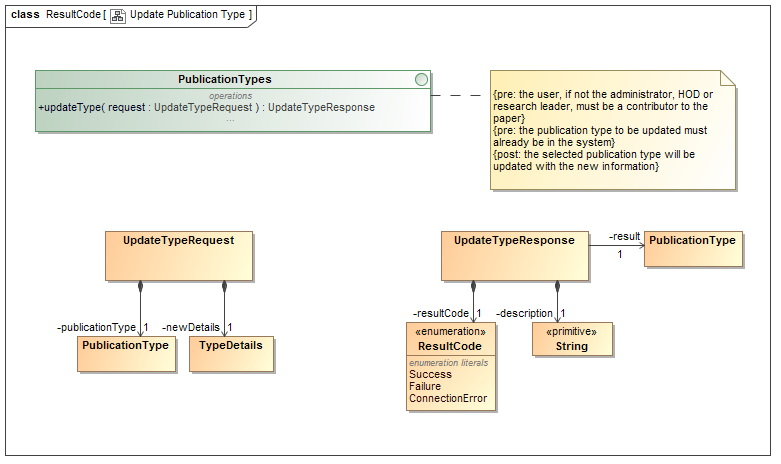
\includegraphics[width=\textwidth]{../Assignment1/5.1.9.Update.Publication.Type.Services.Contract.png}
		\caption{Service Contract: Update Publication}
	\end{figure}
	
	\pagebreak
	\subsubsection{Add Reminder}
	\textbf{Description:} Allows the user to create a reminder for the deadline of the publication.\\
	\textbf{Prioritisation:} Nice-To-Have.
	\\
	
	\textbf{Pre-conditions}
	\begin{itemize}
		\item The user(can be the HOD) should be logged into the system.
		\item The user must be a contributor to the paper.
		\item The publication must already be in the system.
	\end{itemize}
	
	\textbf{Post-conditions}
	\begin{itemize}
		\item A reminder via Mail or Calendar will be set with the selected publication and deadline.
	\end{itemize}
	
	\begin{figure}[H]
		\centering
		%                		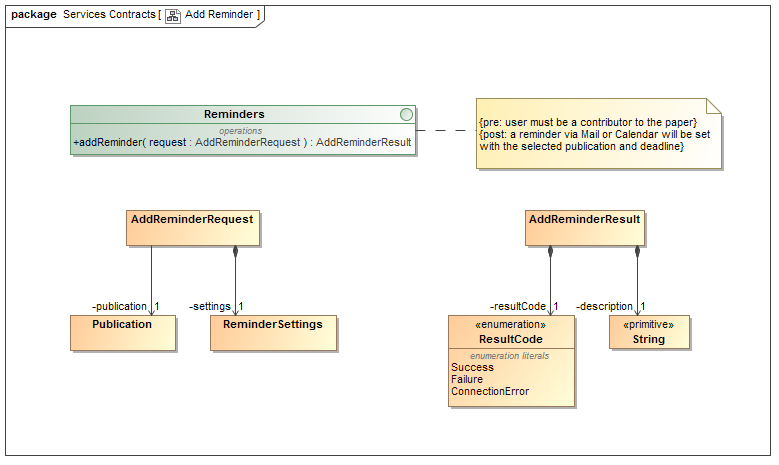
\includegraphics[width=\textwidth]{../Assignment1/5.1.10.Add.Reminder.Services.Contract.png}
		\caption{Service Contract: Add Reminder}
	\end{figure}
	
	\pagebreak
	\subsubsection{Create Research Group}
	\textbf{Description:} Allows the administrator or HOD to create a new Research Group\\
	\textbf{Prioritisation:} Critical\\
	
	\textbf{Pre-conditions}
	\begin{itemize}
		\item The user(must be the administrator or HOD) should be logged into the system.
		\item The Research Group you wish to create must not already be in the system.
	\end{itemize}
	
	\textbf{Post-conditions}
	\begin{itemize}
		\item The Research Group will be created and stored in the database.
		\item Users will be able to join the Research Group.
		\item Research Leader will be able to see all Publications made by the Research Group's members.
	\end{itemize}
	
	\begin{figure}[H]
		\centering
		%    	    		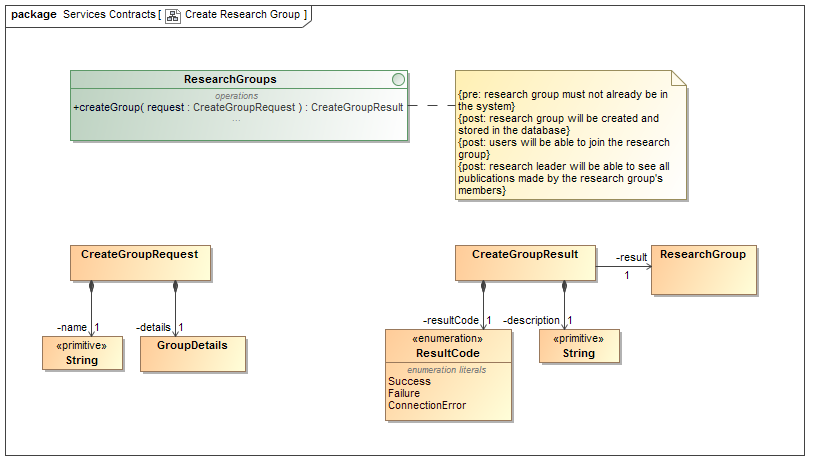
\includegraphics[width=\textwidth]{../Assignment1/5.1.11.Create.Research.Group.Services.Contract.png}
		\caption{Service Contract: Create Research Group}
	\end{figure}
	
	\pagebreak
	\subsubsection{View Research Group}
	\textbf{Description:} View the details of a Research Group \\
	\textbf{Prioritisation:} Nice-To-Have\\
	
	\textbf{Pre-conditions}
	\begin{itemize}
		\item The user(must be the administrator or HOD) should be logged into the system.
		\item The Research Group must already exist in the database.
	\end{itemize}
	
	\textbf{Post-conditions}
	\begin{itemize}
		\item The user will be able to view the details of the Research Group.
	\end{itemize}
	
	\begin{figure}[H]
		\centering
		%    	    		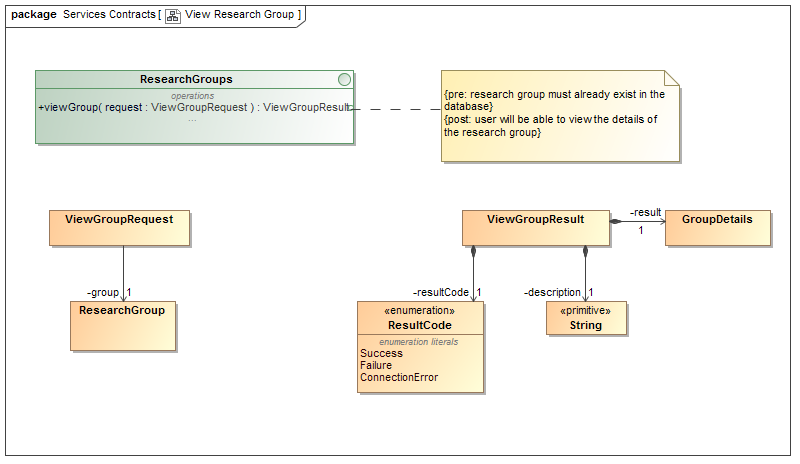
\includegraphics[width=\textwidth]{../Assignment1/5.1.12.View.Research.Group.Services.Contract.png}
		\caption{Service Contract: View Research Group}
	\end{figure}
	
	\pagebreak
	\subsubsection{Update Research Group}
	\textbf{Description:} Allows the administrator or HOD to update an existing Research Group\\
	\textbf{Prioritisation:} Important\\
	
	\textbf{Pre-conditions}
	\begin{itemize}
		\item The user(must be the administrator or HOD) should be logged into the system.
		\item The Research Group must already exist in the database.
	\end{itemize}
	
	\textbf{Post-conditions}
	\begin{itemize}
		\item The user will be able to edit and save the new information entered.
	\end{itemize}
	
	\begin{figure}[H]
		\centering
		%	    		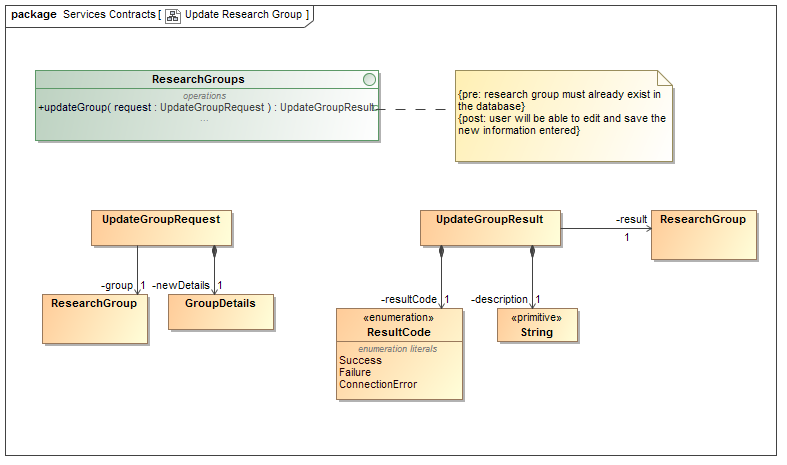
\includegraphics[width=\textwidth]{../Assignment1/5.1.13.Update.Research.Group.Services.Contract.png}
		\caption{Service Contract: Update Research Group}
	\end{figure}
	
	\pagebreak
	\subsubsection{Remove Research Group}
	\textbf{Description:} Allows the administrator or HOD to remove an existing Research Group\\
	\textbf{Prioritisation:} Important\\
	
	\textbf{Pre-conditions}
	\begin{itemize}
		\item The user(must be the administrator or HOD) should be logged into the system.
		\item The Research Group must already exist in the database.
		\item The Research Group must have no members in it and no Research Leader.
	\end{itemize}
	
	\textbf{Post-conditions}
	\begin{itemize}
		\item The user will be able to remove the Research Group from the database.
	\end{itemize}
	
	\begin{figure}[H]
		\centering
		%    	    		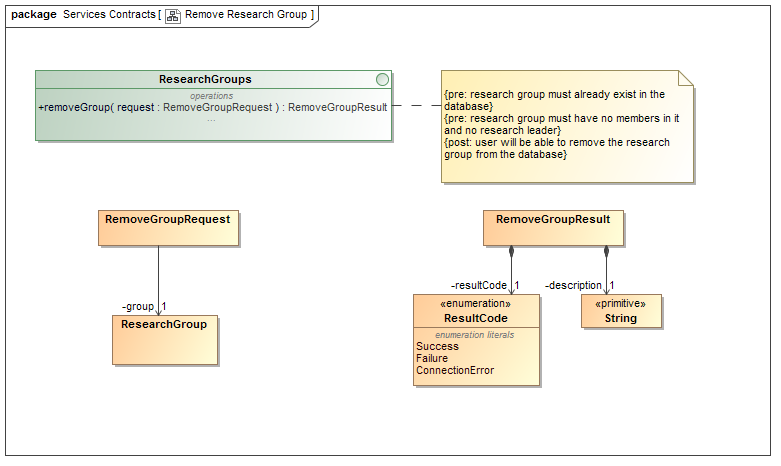
\includegraphics[width=\textwidth]{../Assignment1/5.1.14.Remove.Research.Group.Services.Contract.png}
		\caption{Service Contract: Remove Research Group}
	\end{figure}
	
	\pagebreak
	\subsubsection{Create Author}
	\textbf{Description:} Allows the user to create a new Author\\
	\textbf{Prioritisation:} Critical\\
	
	\textbf{Pre-conditions}
	\begin{itemize}
		\item The user should be logged into the system.
		\item The Author must not already exist in the database.
	\end{itemize}
	
	\textbf{Post-conditions}
	\begin{itemize}
		\item The user will be able to create a new Author and save him/her in the database.
	\end{itemize}
	
	\begin{figure}[H]
		\centering
		%    	    		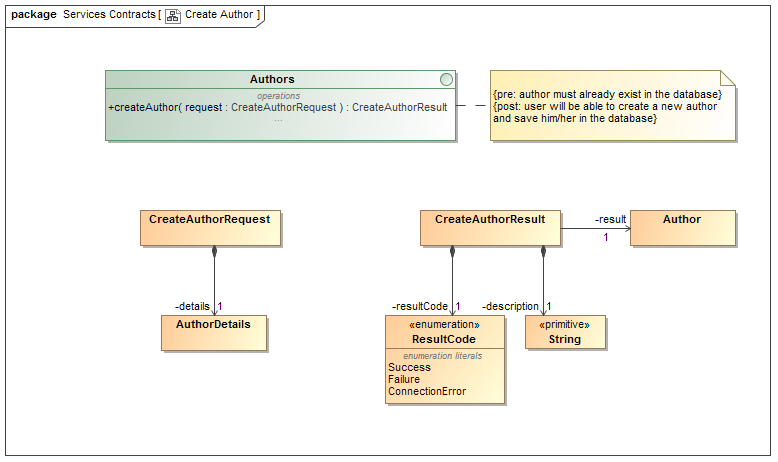
\includegraphics[width=\textwidth]{../Assignment1/5.1.15.Create.Author.Services.Contract.png}
		\caption{Service Contract: Create Author}
	\end{figure}
	
	\pagebreak
	\subsubsection{Update Author}
	\textbf{Description:} Allows the user to update an existing Author\\
	\textbf{Prioritisation:} Important\\
	
	\textbf{Pre-conditions}
	\begin{itemize}
		\item The user should be logged into the system.
		\item The Author must already exist in the database.
	\end{itemize}
	
	\textbf{Post-conditions}
	\begin{itemize}
		\item The user will be able to edit and save the new information entered.
	\end{itemize}
	\begin{figure}[H]
		\centering
		%	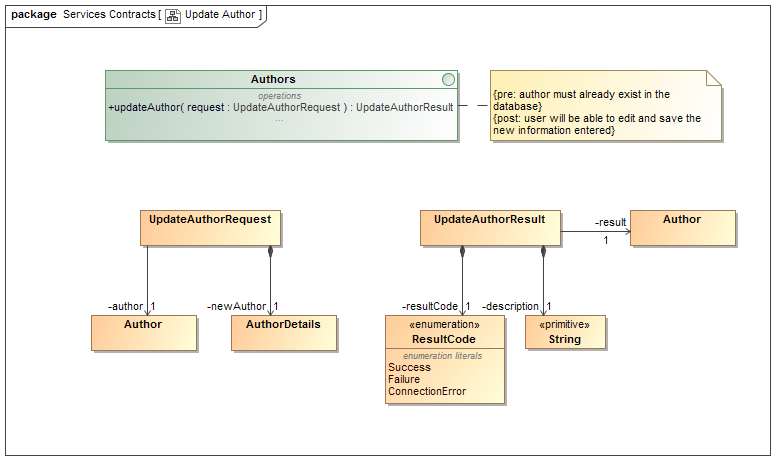
\includegraphics[width=\textwidth]{../Assignment1/5.1.16.Update.Author.Services.Contract.png}
		\caption{Service Contract: Update Author}
	\end{figure}
	
	\pagebreak
	\subsubsection{Generate Report}
	\textbf{Description:} Allows the user generate a report based on certain data\\
	\textbf{Prioritisation:} Nice to have\\
	
	\textbf{Pre-conditions}
	\begin{itemize}
		\item The user should be logged into the system.
		\item There should be existing data in the system's database
	\end{itemize}
	
	\textbf{Post-conditions}
	\begin{itemize}
		\item The system will generate a report based on certain criteria and make it visible to the user
	\end{itemize}
	\begin{figure}[H]
		\centering
		%  		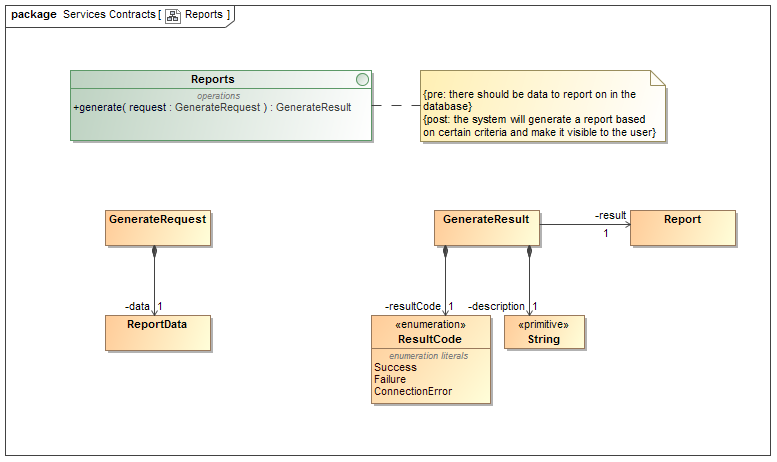
\includegraphics[width=\textwidth]{../Assignment1/5.1.17.Generate.Report.Services.Contract.png}
		\caption{Service Contract: Generate Report}
	\end{figure}
	
	\pagebreak	
	\subsection{Required Functionality}
	\subsubsection{User-Research System interaction}
	\paragraph{\textbf{Description:} The type of user indicates what privileges that user has in the Research system}
	\paragraph{\textbf{Normal-user}}
	\begin{description}
		\item[$\bullet$] A normal user may log in to the system if registered on the system.
		\item[$\bullet$] A normal user may add publications to the system.
		\item[$\bullet$] A normal user must be an author of a publication should they want to add it to the system.
		\item[$\bullet$] A normal user may add authors to a publication.
		\item[$\bullet$] A normal user may change authors in a publication.
		\item[$\bullet$] A normal user may add a publication to a conference.
		\item[$\bullet$] A normal user may only view their own publications.
	\end{description}
	\paragraph{\textbf{Head of Department}}
	\begin{description}
		\item[$\bullet$] The head of department may log in to the system.
		\item[$\bullet$] The head of department may add/edit/remove a user.
		\item[$\bullet$] The head of department may add/edit/remove an author.
		\item[$\bullet$] The head of department may add publication/edit a publication.
		\item[$\bullet$] The head of department may be an author on a publication.
		\item[$\bullet$] The head of department may add authors to a publication.
		\item[$\bullet$] The head of department may add/remove publications for conferences.
		\item[$\bullet$] The head of department may view all publications on the system.
	\end{description}
	\paragraph{\textbf{Admin}}
	\begin{description}
		\item[$\bullet$] Admin users may log in to the system.
		\item[$\bullet$] Admin users may add/remove/edit users.
		\item[$\bullet$] Admin users may add/edit publications.
		\item[$\bullet$] Admin users may not be an author to any publication on the system.
		\item[$\bullet$] Admin users may add authors to a publication.
		\item[$\bullet$] Admin users may change authors to a publication.
		\item[$\bullet$] Admin users may add/remove publications to conferences.
		\item[$\bullet$] Admin users may view all publications on the system.
	\end{description}
	\begin{figure}[H]
		%		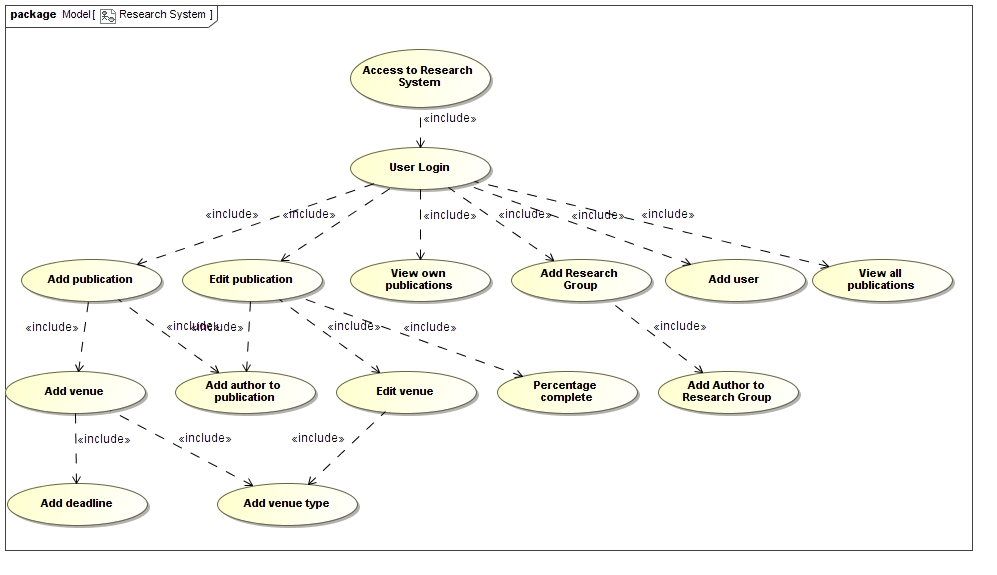
\includegraphics[width=\textwidth]{../Assignment1/Overview.jpg}
		\caption{Functional Requirements: Overview of Research System \label{overflow}}
	\end{figure}
	\begin{figure}[H]
		%		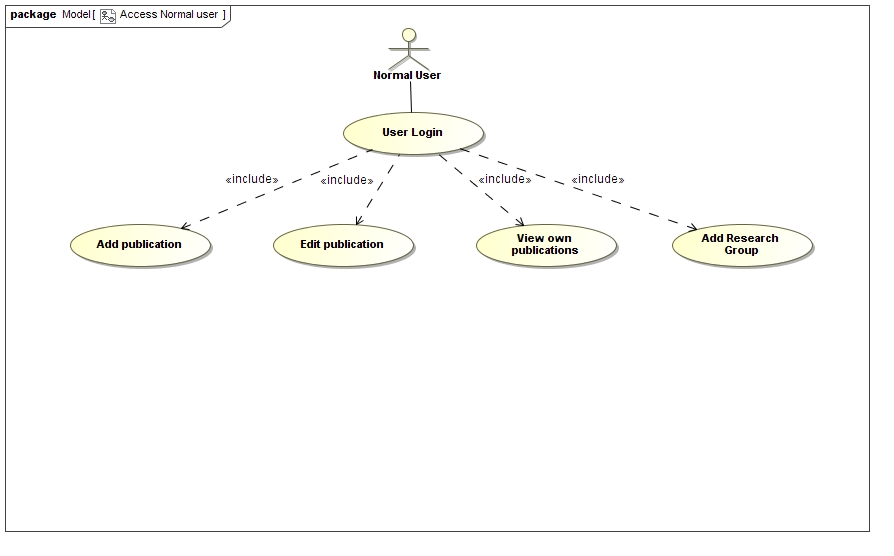
\includegraphics[width=\textwidth]{../Assignment1/AccessNormaluser.jpg}
		\caption{Functional Requirements: Normal user access privileges \label{overflow}}
	\end{figure}
	\begin{figure}[H]
		%		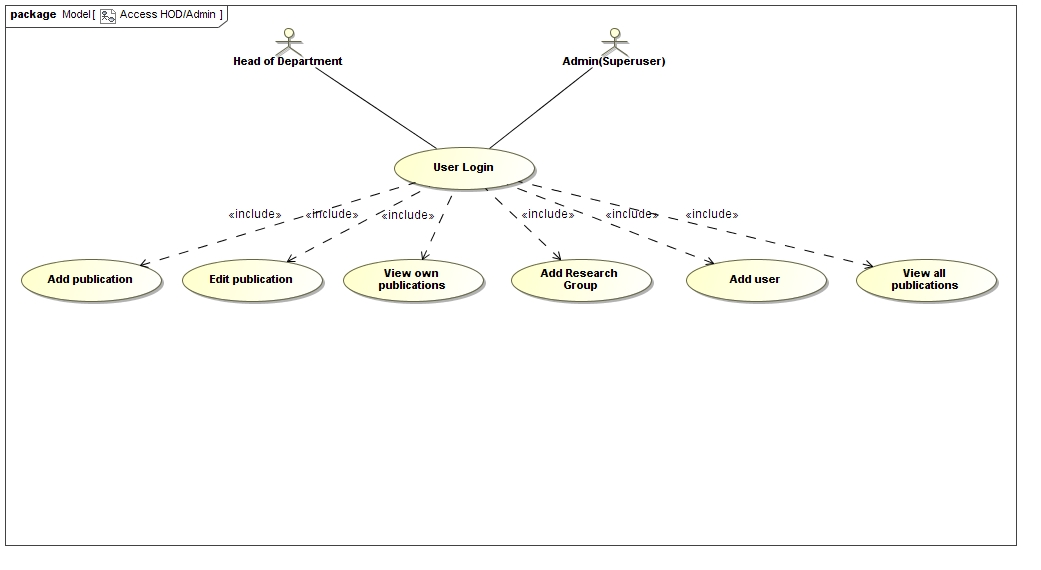
\includegraphics[width=\textwidth]{../Assignment1/AccessHODAdmin.jpg}
		\caption{Functional Requirements: Superuser(HOD and admin) access privileges \label{overflow}}
	\end{figure}
	\pagebreak
	\subsection{Process Specification}
	This section conatins UML activity diagrams that illustrate the sequences that will be followed for various use case scenarios.
	\begin{figure}[H]
		\centering
		%	    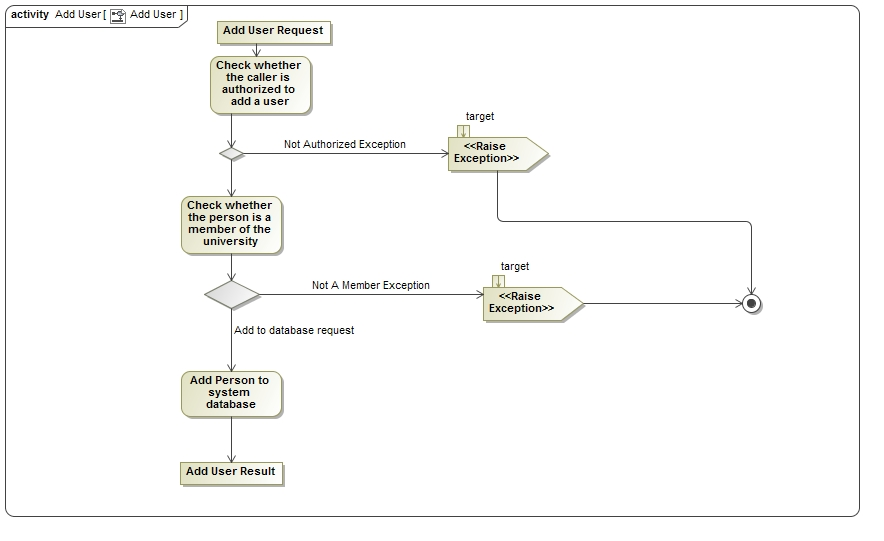
\includegraphics[width=\textwidth]{../Assignment1/AddUser.jpg}
		\caption{Process Specification: Adding A User}
	\end{figure}
	\begin{figure}[H]
		\centering
		%	    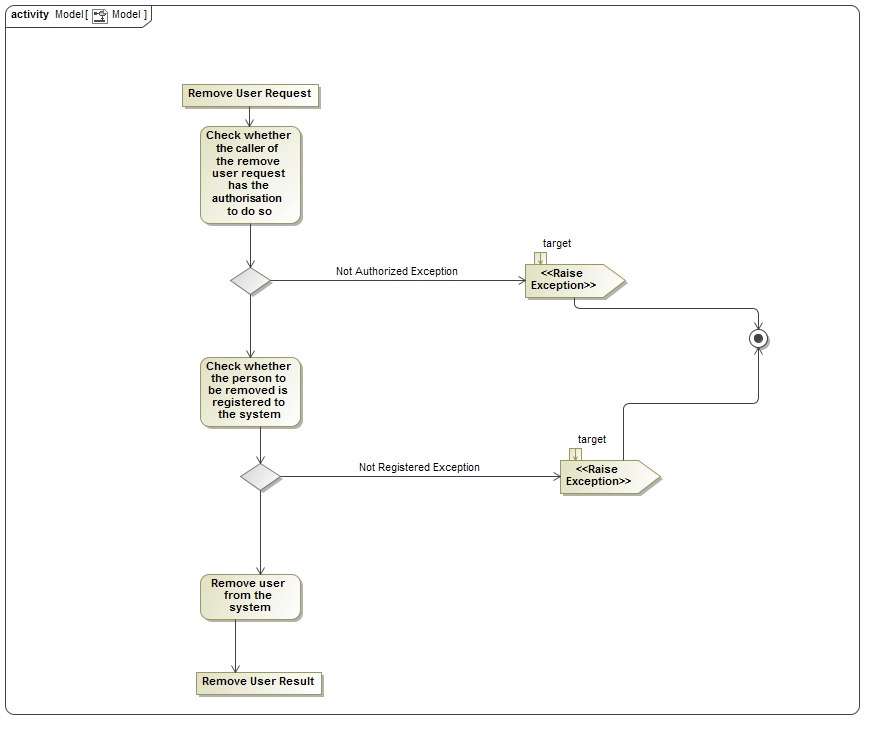
\includegraphics[width=\textwidth]{../Assignment1/removeUser.jpg}
		\caption{Process Specification: Removing A User}
	\end{figure}
	\begin{figure}[H]
		\centering
		%	    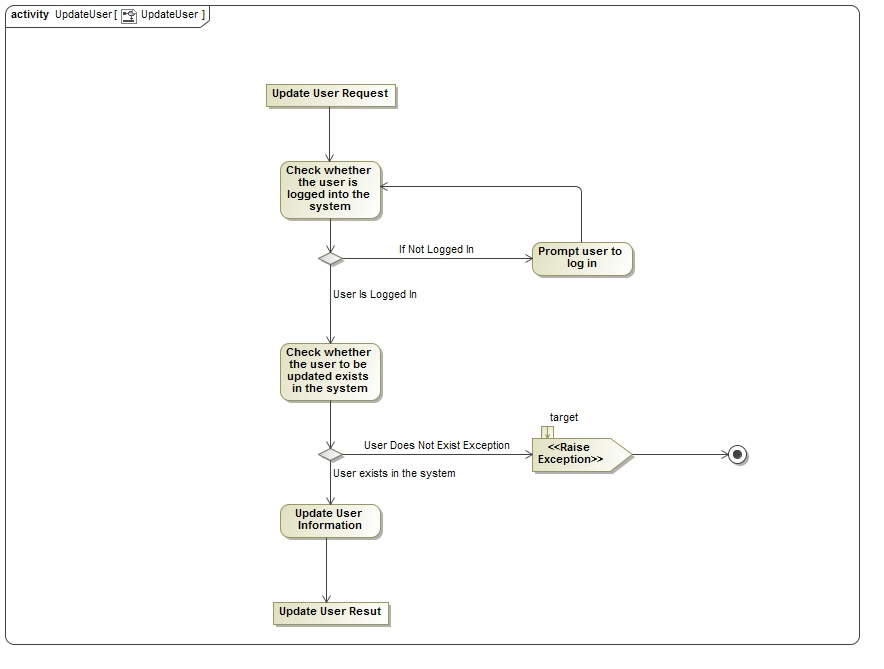
\includegraphics[width=\textwidth]{../Assignment1/UpdateUser.jpg}
		\caption{Process Specification: Update A User}
	\end{figure}
	\begin{figure}[H]
		\centering
		%	    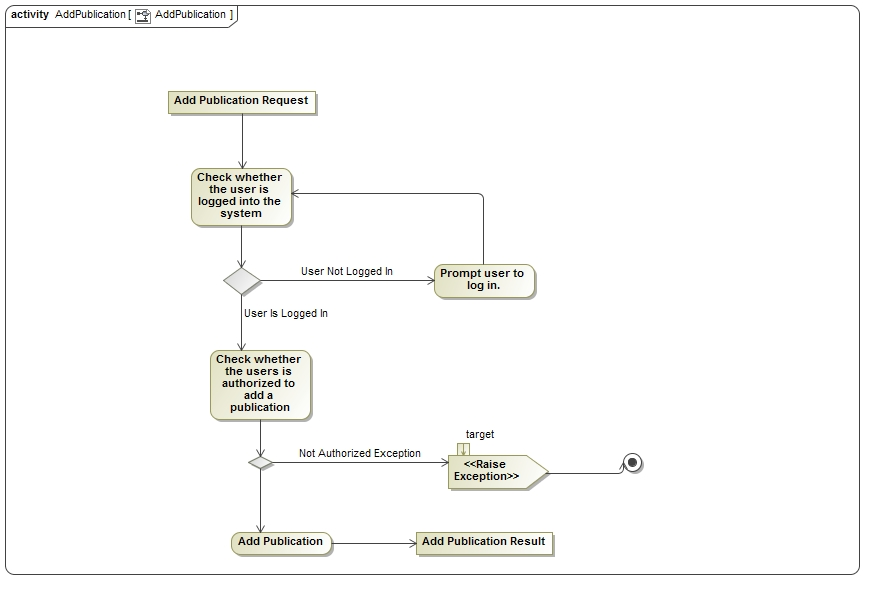
\includegraphics[width=\textwidth]{../Assignment1/AddPublication.jpg}
		\caption{Process Specification: Adding A Publication}
	\end{figure}
	\begin{figure}[H]
		\centering
		%	    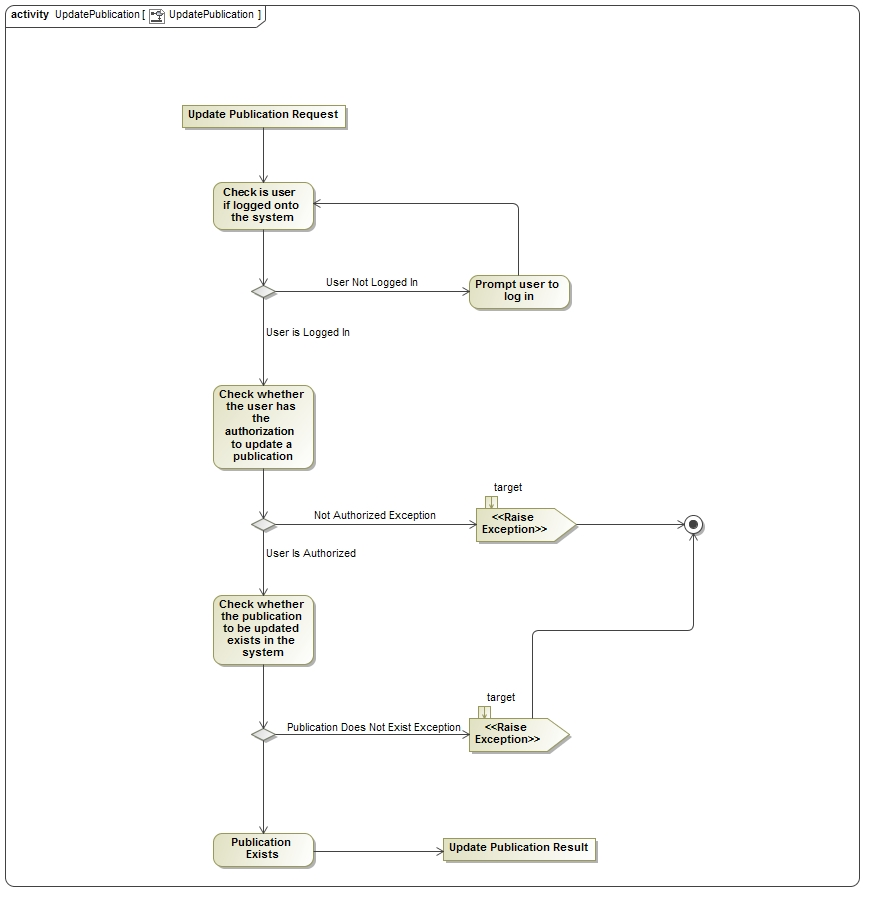
\includegraphics[width=\textwidth]{../Assignment1/UpdatePublication.jpg}
		\caption{Process Specification: Update A Publication}
	\end{figure}
	\begin{figure}[H]
		\centering
		%	    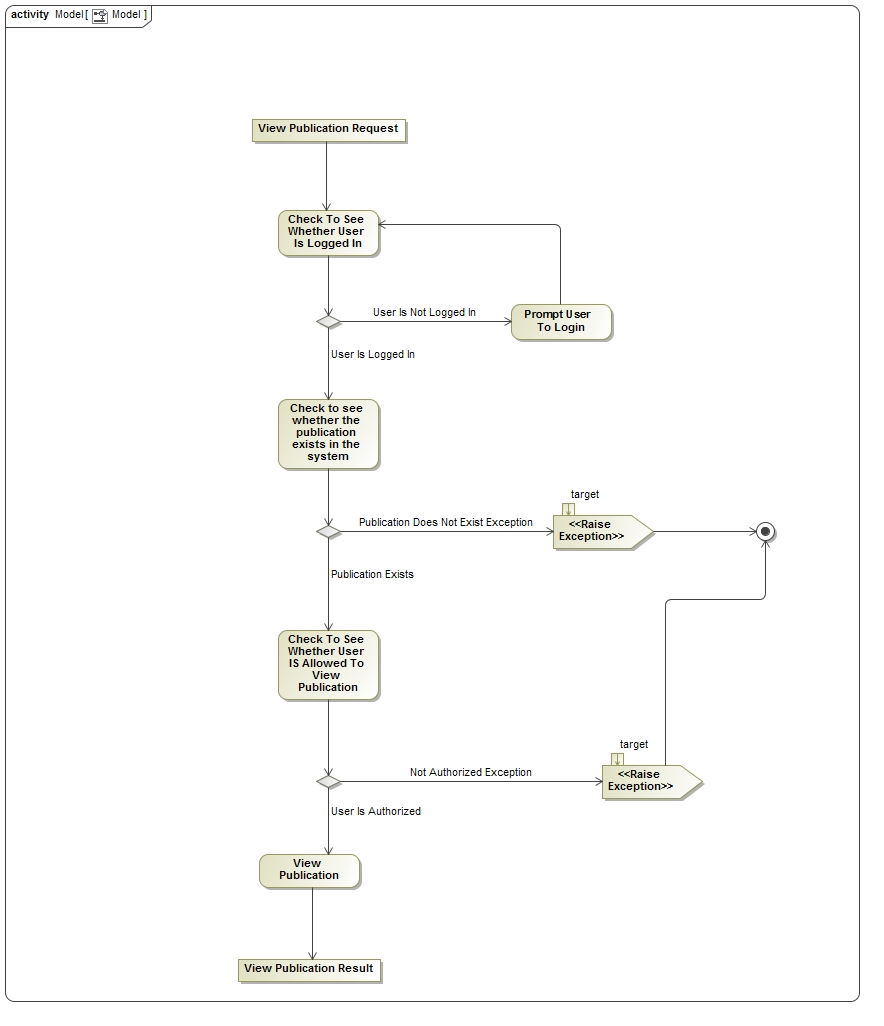
\includegraphics[width=\textwidth]{../Assignment1/ViewPublication.jpg}
		\caption{Process Specification: View A Publication}
	\end{figure}
	\subsection{Domain Model}
	\begin{figure}[H]
		%		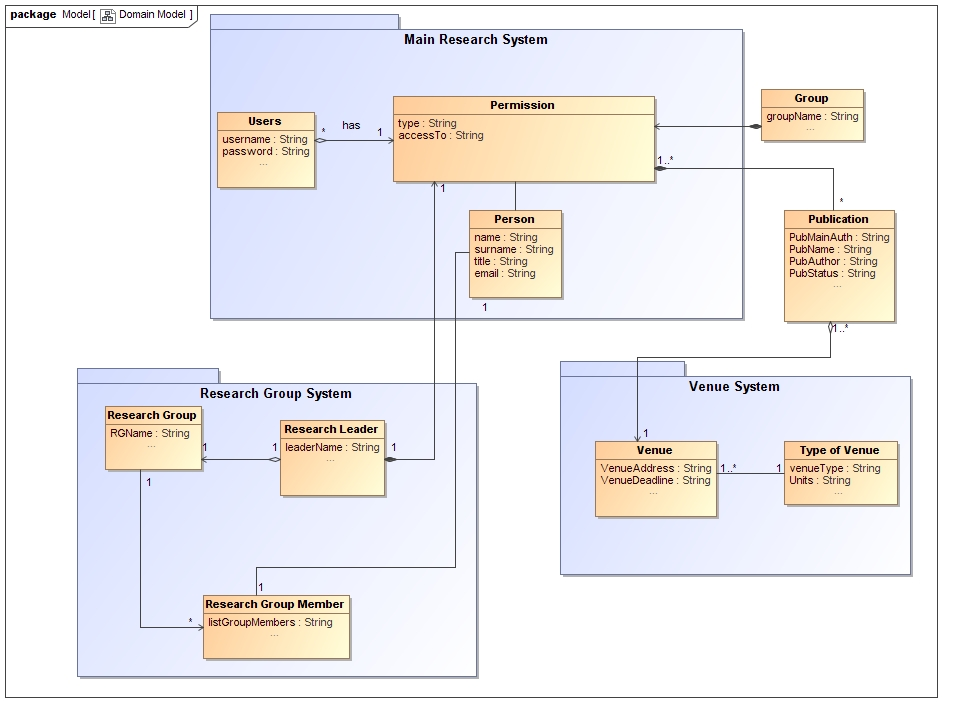
\includegraphics[width=\textwidth]{../Assignment1/DomainModel.jpg}
		\caption{Domain Model of Research System \label{overflow}}
	\end{figure}
	\pagebreak
	\section{Open Issues}
	This section deals with issues that still need to be clarified, specified, assumed or have been discovered to include inconsistencies in the requirements, comprising of the following issues:
	\begin{description}
		\item[$\bullet$] Will a server be provided?
	\end{description}
	\begin{description}
		\item[$\bullet$] Should the HOD be a separate entity or fall within the Admin entity?
	\end{description}
	\begin{description}
		\item[$\bullet$] To where does the publication go to be reviewed?
	\end{description}
	\begin{description}
		\item[$\bullet$] Should the reminder system be via Mail or Calendar notification?
	\end{description}
	\begin{description}
		\item[$\bullet$] It is assumed that the Venue will have a deadline attached.
	\end{description}
	
\end{document}
=======
\documentclass[a4paper]{article}

%opening

\title{\huge Functional Requirements And Software Architecture Specification
	\\COS 301 Team Alpha Project
	\\Version 2.0}

\author{\\\\Amy Lochner 14038600\\ Avinash Singh 14043778 \\
	Christiaan Nel 14029368\\ Christiaan Saaiman 12059138 \\
	Gerard van Wyk 14101263\\ Marc Antel 12026973\\
	Themba Mbhele 14007950
	\\
	\\
	\\\textit{https://github.com/AvinashSingh786/COS301-Alpha.git}
	\\
	\\
	\\ University Of Pretoria\\}

\date{March 2016}

\usepackage{graphicx}
\usepackage{float}
\usepackage{hyperref}
\begin{document}
	
	\maketitle
	
	\pagenumbering{gobble}
	\newpage
	
	\tableofcontents
	\pagenumbering{arabic}
	\newpage
	
	\section{Introduction}
	
	This document defines the Software Requirements Specification and Technology Neutral Process Design for COS 301 Team Alpha. The Computer Science Department has expressed a need for the creation of a system, which can allow researchers to keep track of publications which they are currently working on, or have already published.
	\\
	The aim of this project is to follow a structured software development process in order to produce a product which provides the client with all the required functionality in an elegantly designed and built product. A collaborative and co-operative approach is required between all stakeholders who are involved in this project. 
	\\
	The information, specifications, and diagrams within this document are presented in order to provide testable requirements which correlate to the client's needs.
	
	\section{Vision}
	The client for this project, Ms. Vreda Pieterse who is a member of the Department of Computer Science at the University of Pretoria, has solicited us to develop a system. The purpose of this system is to record and oversee all publications of staff members or research groups, within the Department of Computer Science. The system will assist the Head of Department to track the progress on any papers which are in the process of being written; as well as determining whether or not a staff member is under performing thus allowing the Head of Department the opportunity to provide advice to these staff members.
	
	\section{Background}
	\subsection{The client's problem}
	The client has solicited us to develop a system that has specific usability goals, as well as certain user-experience goals. Currently, the Department of Computer Science does not have a system with which to monitor the progress of staff member's publications, nor to keep track of how many publications an author is working on. Furthermore, it is necessary to determine which publications will be presented at different conferences, as well as the reporting capabilities, and the ability to remind users of deadlines. The system should provide all these requirements in a secure, flexible and intuitive manner.
	
	
	\subsection{Future business/research opportunities}
	It is desired that this system will encourage authors to collaborate with other authors on similar topics and to expand the users base knowledge of ongoing research projects.
	\\
	\\
	\\
	
	
	\section{Software Architecture Documentation}
	
	This document defines 
	
	\subsection{Architecture requirements}
	In this section extract the architectural requirements from the software requirements, including:
	
	\subsubsection{Architectural Scope}
	Architectural responsibilities that need to be addressed by the software architecture are as follows:
	\begin{itemize}
		\item Providing a persistent infrastructure - being a database stored on a dedicated server
		\item Providing a reporting infrastructure
		\item Providing an infrastructure for process execution
		\item Providing a backup infrastructure (e.g. making use of RAID)
		\item Providing a user interface through which the user can interact with the website/app
		\item Providing a means of Session management
		\item Providing a method of prevention against SQL injections
		\item Provide a log in system
		\item Provide a means with which to query the database in an interactive way
		\item Provide a means by which users can be notified about reminders
	\end{itemize}
	\subsubsection{Quality requirements}
	\begin{itemize}
		\item Performance \\\\
		The performance of a system refers to the behaviour of the system in terms of repsonse time and throughput. Changes and modifications to the system should be done in the most cost and time effective manner to provide a good user experience.
		One method of ensuring the performance is visible to the user is to make use of feedback tools to ensure the user is aware that the system is performing as expected or to notify the users should something have gone wrong.  
		\item Security \\\\
		Minimising the possibility of leaking information, maintaining data integrity, and avoiding session hijacking. This is very important as personal information will be stored in the database(e.g. email). The system will also have different user types with different access permissions hence security will be needed to ensure that a specific user only has the capabilities afforded to them. 
		\\\\
		We will achieve security by making use of 3 methods, namely: prevention, detection, and recovery.
		We will ensure that we have put means in place through which we may be able to detect any threats to the system, for example validating any information that is required to be sent to the server. Preventing threats to the system can be enforced through limiting the access channels, making use of authentication, not allowing any external sources to be accessed through the system, etc. Recovery will be achieved through cancelling requests and maintaining a working back up state to reroll changes.
		\item Maintainability \\\\
		This refers to how well the system can be modified to accommodate new functionality, access channels, fix bugs and improve the performance of the system. As it is likely that multiple people will be working on the system the code has to be easy to read and understand. We will achieve this by commenting our code to allow for a quick study of the code. We will employ a means by which to allow pluggability of our code to ensure that large amounts of code will not be needed to be changed/removed.
		\\\\
		The system should not only be maintainable in terms of issues with the system but it should also be maintainable in terms of usability, i.e user permissions should be allowed to be changed, etc.
		
		\item Scalability \\\\
		Scalabilty refers to the system's ability to handle increased traffic or workload. This will be implemented by ensuring that users can make the same requests simultaneously.
		\\\\
		We will need to ensure that resources are managed wisely in order to avoid lost updates, uncommitted data and inconsistent retrievals.
		
		\item Reliability \\\\
		As the system is required to support a fairly large user base it should allow for effective and safe concurrent use of the system. The system should ensure that no users can perform tasks that their user type does not afford to them.
		\\\\
		As access channels are via a web browser/android app it is essential that these access channels always have access to the server and thus database and ensure that the connection is stable, reliable and safe at all times. The system should be maintained in order to ensure that the system can perform all the required tasks in an effective and efficient manner. We will achieve this through unit testing, making use of concurrent resource locks and eliminating single points of failure.
		\item Auditability\\\\
		A requirement of the system is that all actions or changes to the should be logged to enable users with the appropriate permissions to be able to view all actions or changes to the system, who they were made by and when. This is essential in ensuring that the system can be rolled back to a stable state should something undesirable happen.
		\\\\
		We will implement this by having a log file running at all times which makes use of timestamping to indicate when changes were made, the system should allow to be rolled back to a stable state should it be deemed neccessary. ACID Properties will be applied to ensure that the database maintains a stable, reliable and current state.
		
		
		\item Integrability \\\\
		Will the system be able to integrate with other technologies.
		\item Usability \\\\
		Usability will be achieved through the implementation of an intuitive, easy to use, easy to understand and an aesthetically appealing interface through which the user will be able to perform all system functionality afforded to them through their user type.
		\\\\
		We will ensure that the user interface performs all tasks in the most efficient and direct means. The interface should not cause the user any irritation in the form of colour schemes, delayed functionality, over complication of tasks.
	\end{itemize}
	
	
	\subsection{Integration and access channel requirements}
	The CS Research System will serve as the basis of the entire system, possibly integrating with future systems. Integration can be made possible through the use of a RESTful API to enable cross-platform concurrent communication through HTTP or HTTPS. By using a service-oriented architecture and thereby componentizing the system, other systems can more easily integrate through service calls to these different components. A web interface as well as a mobile application, specifically on Android, should be made available for the end users. Other platforms should then be able to communicate with the system through simple REST API calls. Additionally, services such as Google Calendar and Google Mail can also be integrated into the system through simple API calls made available by Google. 
	\\
	
	\subsubsection{Architectural constraints}
	It is desired that this system will encourage authors to collaborate with other authors on similar topics and to expand the users base knowledge of ongoing research projects.
	\\
	\\
	\\
	
	
	\section{Architectural patterns or styles}
	Architectural Patterns are generally reusable solutions to commonly occuring problems within a given context. Similar to software design patterns, architectural patterns are 
	larger in scope though. The architectural patterns address various problems such as:
	\begin{itemize}
		\item Software Engineering
		\item Computer Hardware limitations
		\item High availablility
		\item Minimization of Business Risk
	\end{itemize}
	
	For this project and the scope thereof, I suggest either one of two architectures are used or possibly both.
	\subsection{Model-View-Controller}
	Model-View-Controller, here on out referred to as MVC, is popular architecture used for implementing systems with user-interfaces. Later this architecture
	became extremely popular for designing web applications and for this reason I suggest using this architecture. This architecture is easy to implement and 
	to maintain. It is divided into three seperate departments:
	\begin{itemize}
		\item The Model is in charge of managing the data, logic and rules of the system.
		\item The view is responsible for outputting the representation of the data that the user perceives.
		\item The controller takes in input and converts it to commands for the model & view.
	\end{itemize}
	Current day MVC architecture has moved away from thin client coding due to technologies such as AngularJS, EmberJS, JavaScriptMVC and Backbone.
	
	\subsection{Service-orientated Architecture}
	A service-oriented architecture (SOA) is an architectural pattern in computer software design in which application components provide services 
	to other components via a communications protocol, typically over a network. The principles of service-orientation are independent of any vendor, 
	product or technology.
	
	A service is a self-contained unit of functionality, such as retrieving an online bank statement. By that definition, a service is an operation
	that may be discretely invoked. However, in the Web Services Description Language (WSDL), a service is an interface definition that may list several
	discrete services/operations. And elsewhere, the term service is used for a component that is encapsulated behind an interface. This widespread
	ambiguity is reflected in what follows.
	
	Services can be combined to provide the functionality of a large software application. SOA makes it easier for software components on computers
	connected over a network to cooperate. Every computer can run any number of services, and each service is built in a way that ensures that the service
	can exchange information with any other service in the network without human interaction and without the need to make changes to the underlying program
	itself.
	
	\section{Architectural tactics or strategies}
	In this section, we will discuss certain strategies that will be used to achieve the quality requirements stated in section 4.2 and were further expanded upon in section 5.1.2.
	\begin{itemize}
		
		
		\item Hashing and Salting Passwords \\\\
		To ensure that sensitive information of the users of the system is not leaked in the event of a database compromise, all passwords will not be stored in plain text. Instead, all passwords will be hashed with a strong one-way hashing algorithm, such as the sha256, so that in the event of a database compromise, it will be near impossible to compute the actual passwords from the hashes. To make the hashes more effective, we will add random data, known as salt, to the passwords before hashing them. This will make it extremely difficult for intruders to use pre-hashed tables to perform a look up to find a matching password.
		\\
		\item Prepared Statements \\\\
		To prevent the illegal extraction of data and/or the destruction of data from the database through SQL injection and blind SQL injection attacks, we will make use of prepared statements. Prepared statements also have other benefits other than security. Even though prepared statements execute a statement multiple time, they reduce parsing time as the preparation of the query is only done once. This will improve the efficiency and performance of the system. Also, because prepared statements bind values to parameters, the bandwidth on the server is minimized because you only need to send the parameters to the server and not the whole query. This also improves the performance of the system.
		\\
		\item Caching \\\\
		Because the system relies heavenly on databases, there will be a significant number of access attempts to the the databases. This has the potential of creating a bottleneck that gets worse as the number of concurrent users increases. This means that the system will scale poorly and the performance of the system will decrease drastically. The best way to combat this is to limit accesses to the databases were possible. To accomplish this, we will make use of a distributed cache system. A distributed cache will particularly be effective in read operations and will provide large performance gains as it reduces the processing times of applications and it limits database accesses. This will improve the scalability of the system drastically and thus will accommodate a large number of concurrent users. 
		\\
		\item Database Normalization \\\\
		To make the system flexible, we will create the database tables and link them to one another were it is appropriate to do so according to rules that protect the data and makes it flexible. This process is known as normalization. Normalization eliminates redundancies and inconsistent dependencies. This makes it simple to makes changes to the system and also makes it easy to add new components to the system.
		\\
	\end{itemize}
	\section{Use of reference architectures and frameworks}
	\section{Access and integration channels}
	The following is a tentative list of the access/integration channels planned for use in the final architecture. The word "tentative" is used as we cannot say with complete certainty what will be used before actual programming for the architecture has started to be written.
	
	\begin{itemize}
		\item The Web protocols to be used: 
		HTTP, HTTPS, FTP.
		\item API - UML Interfaces.
		A proprietary object-relational mapper will be developed to manage the conversion of data-objects across different programming languages where necessary, this could be as simple as a java program that takes language A's object, converts it to a .txt file, then builds a language B object from it, or it could involve some third party object-relational mapper, whatever works.
		\item Google Calender and Email integration.
		Any event in the database that has a date/time must be sent to any person semantically involved with that event.
		The relevant people will have the event automatically placed on their Google Calendar, and they will receive an automated email notifying them of the event once when the event is created, and once when the date of the event draws near. Various Google APIs/libraries will assist in acheiving this.
		\item Web-and Mobile functionality Integration.
		The application must be accesible from both a web portal and from an android app. The Android SDK will most likely be used to resolve all of the android usability goals.
		\item Venue and Publication integration.
		The Google Calender and email integration will contain the necessary Venue and Publication information if applicable.
		\\
	\end{itemize}
	
	
	
	\section{Technologies}
	The following technologies will be used to develop the Research System:
	\begin{itemize}
		\item HTML (Hypertext Markup Language): A standardized system for tagging text files to achieve font, colour, graphic, and hyperlink effects on World Wide Web pages. This will be the interface for the users of the system. 
		\item AJAX (Asynchronous JavaScript and XML): Ajax is a group of interrelated Web development techniques used on the client-side to create asynchronous Web applications. The use of Ajax will bring dynamic changes to the web page. This will update changes to the system without the user having to refresh the page and will avoid identical information being submitted multiple times by multiple users. 
		\item JavaEE (Java Platform Enterprise Edition): This platform provides an API and runtime environment for developing and running enterprise software, including network and web services, and other large-scale, multi-tiered, scalable, reliable, and secure network applications. JavaEE is fundamental for the Research System in providing the connections for the user to the system.
		\item JavaScript (Functionality to HTML): An object-oriented computer programming language commonly used to create interactive effects within web browsers. This will enhance the functionality and appearance of the web pages of the Research System.
		\item PHP (Server Side Scripting): PHP is a server scripting language, and a powerful tool for making dynamic and interactive Web pages. The Research System will use PHP for collecting data from forms, such as adding a user and adding a publication. 
		\item MySQL (Database Manager): MySQL is a database system used on the web, which runs on the server. This will be the chosen database system, since it is very fast, reliable, and easy to use, as well as being able to compile on a number of platforms.
		\item Android (Mobile Devices): Android is a mobile operating system, which is designed primarily for touchscreen mobile devices such as smartphones and tablets. An android application will be developed for the Research System, to provide an easy to use interface for the user on mobile devices.
		\item Apache (Web Server): The Apache HTTP Server is the world's most used web server software. This is the chosen its performance and reliability, as well as being able to support the other technologies that the Research System will be using. 
		\item Linux/Windows/Mac (Operating System): The three operating systems that are most commonly used today. The Research System will have to be able to run in these three Operating Systems.
		\\
		\\
	\end{itemize}
	\pagebreak
	
	
	
	% ==============================================================================================================================================================
	
	
	
	
	
	
	
	
	
	
	
	
	
	
	
	
	
	\section{Functional Requirements and Application Design}
	This section discusses the application functionality and service contracts required by the users.
	\subsection{Use Case Prioritization}
	The Use Case Prioritisation is specified for each use case in the next section.
	
	\subsection{Use Case/Services Contracts}
	Use Case Prioritisation and Service Contracts are described below
	
	\subsubsection{User Login}
	\textbf{Description:}  A user is required to log into the system before the user can make use of any functionality.
	\\
	\textbf{Prioritisation:} Critical\\
	
	
	\textbf{Pre-conditions}
	\begin{itemize}
		\item A user must have a connection to the server.
		\item A user must be registered as a user by a person with HOD or Admin permission.
		\item The user must enter the correct information in order for the authentication to be successful.
	\end{itemize}
	
	\textbf{Post-conditions}
	\begin{itemize}
		\item The user has specific access to the server on which all data is stored, i.e add/edit authors and search for authors
		\item The user is able to use all the user functionality provided by the system 
		\item The user may log out of the system when they wish to.
	\end{itemize}
	
	\begin{figure}[H]
		\centering
		%            		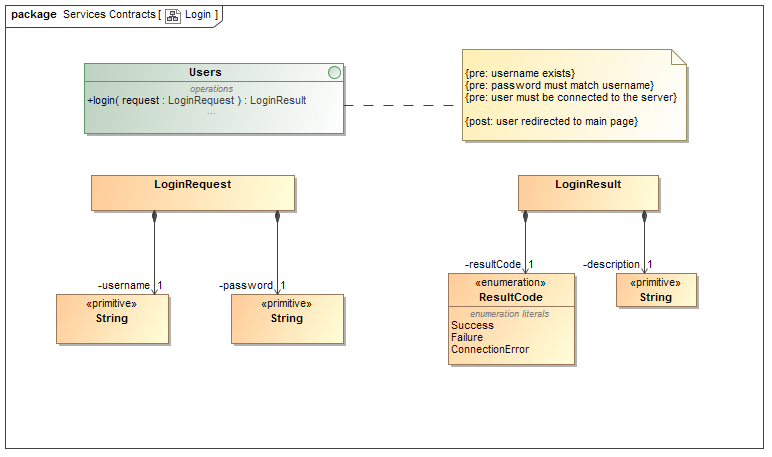
\includegraphics[width=\textwidth]{../Assignment1/5.1.1.Login.Services.Contract.png}
		\caption{Service Contract: User Login}
	\end{figure}
	
	\pagebreak
	\subsubsection{User Registration}
	
	\textbf{Description:}  In order to be able to log into the system and make use of the functionality provided by the system the user must be registered on the system. \\
	\textbf{Prioritisation:} Critical\\
	
	\textbf{Pre-conditions}
	\begin{itemize}
		\item The user must be part of the staff of the Computer Science Department of the University of Pretoria.
		\item The administrator or HOD of the system must have registered the user on the system.
		\item The user must decide on their login credentials.
	\end{itemize}
	
	\textbf{Post-conditions}
	\begin{itemize}
		\item The user's login information is securely stored in the system database.
		\item The user can log into the system.
	\end{itemize}
	
	\begin{figure}[H]
		\centering
		%        		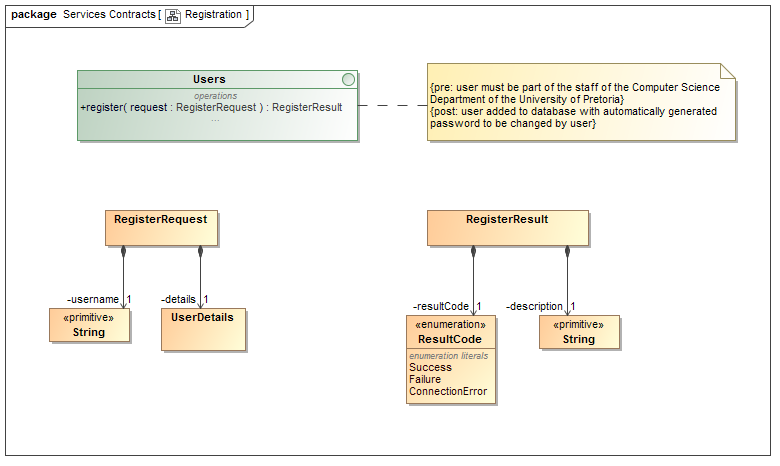
\includegraphics[width=\textwidth]{../Assignment1/5.1.2.Registration.Services.Contract.png}
		\caption{Service Contract: User Registration}
	\end{figure}
	
	
	\pagebreak
	\subsubsection{Update User}
	
	\textbf{Description:} Personal details as well as log in credentials can be changed if and when necessary.\\
	\textbf{Prioritisation:} Important\\
	
	\textbf{Pre-conditions}
	\begin{itemize}
		\item The administrator or HOD must be logged into the system.
		\item The user to be updated must already exist in the system.
		\item The administrator or HOD must have the new information.
	\end{itemize}
	
	\textbf{Post-conditions}
	\begin{itemize}
		\item The user's information is updated on the system's database.
	\end{itemize}
	
	\begin{figure}[H]
		\centering
		%            		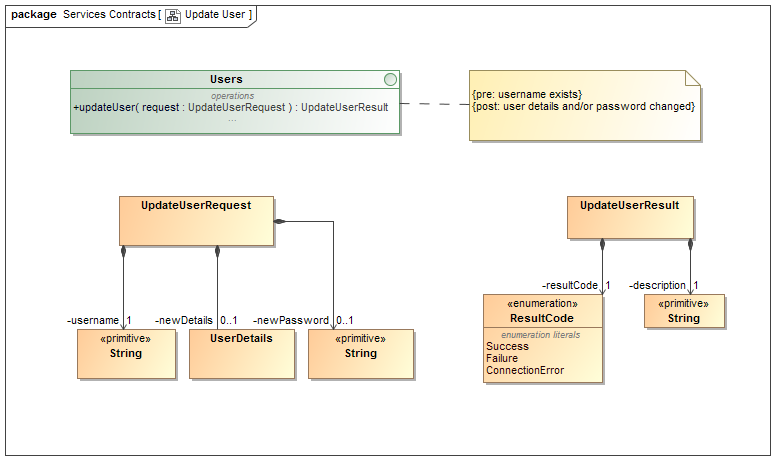
\includegraphics[width=\textwidth]{../Assignment1/5.1.3.Update.User.Services.Contract.png}
		\caption{Service Contract: Update User}
	\end{figure}
	\pagebreak
	\subsubsection{Remove User}
	
	\textbf{Description:} Should a user no longer belong to the Department of Computer Science the person should be removed from the system.\\
	\textbf{Prioritisation:} Important\\
	
	\textbf{Pre-conditions}
	\begin{itemize}
		\item The person should be a user on the system.
		\item The person should no longer belong to the staff of the Department of Computer Science.
		\item The administrator or HOD must be the logged in.
	\end{itemize}
	
	\textbf{Post-conditions}
	\begin{itemize}
		\item The person is removed from the system's database.
		\item The person can no longer gain access to the system.
		\item The person history still remains in the log file.
	\end{itemize}
	
	\begin{figure}[H]
		\centering
		%        		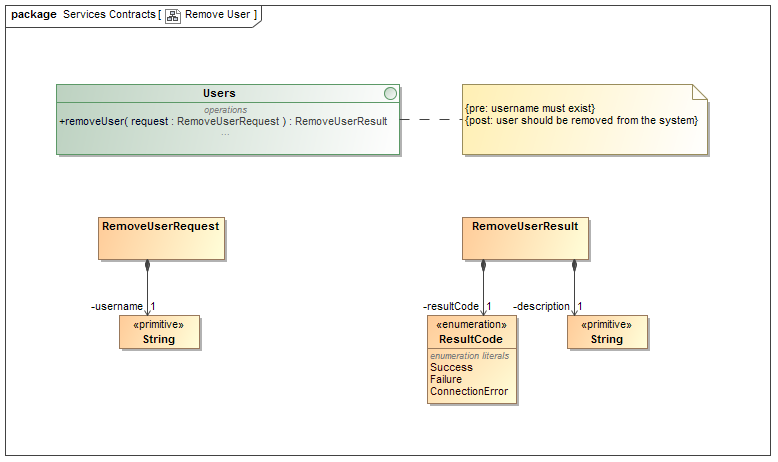
\includegraphics[width=\textwidth]{../Assignment1/5.1.4.Remove.User.Services.Contract.png}
		\caption{Service Contract: Remove User}
	\end{figure}
	\pagebreak
	\subsubsection{Create Publication}
	
	\textbf{Description:} Adding a paper to the system\\
	\textbf{Prioritisation:} Critical\\
	
	
	\textbf{Pre-conditions}
	\begin{itemize}
		\item The user(may be the administrator or HOD) should be logged into the system.
		\item The user, if not the administrator or HOD, must be a contributor to the paper.
		\item All authors who contributed to the paper should be available on the system.
	\end{itemize}
	
	\textbf{Post-conditions}
	\begin{itemize}
		\item The paper is added to the system
	\end{itemize}
	
	\begin{figure}[H]
		\centering
		%            		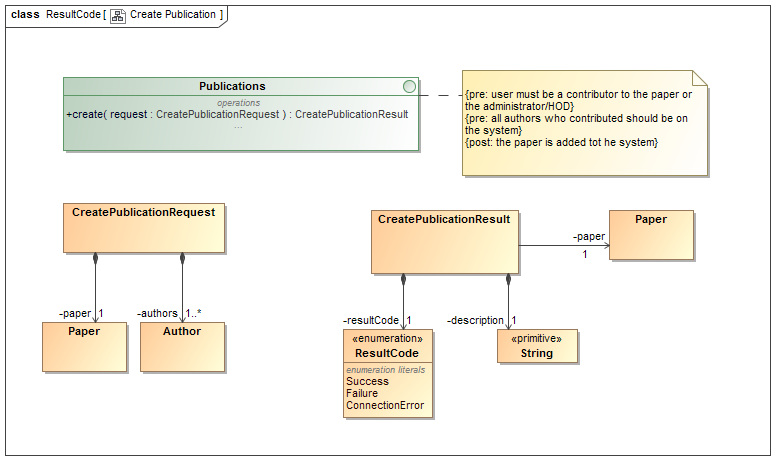
\includegraphics[width=\textwidth]{../Assignment1/5.1.5.Create.Publication.Services.Contract.png}
		\caption{Service Contract: Create Publication}
	\end{figure}
	\pagebreak
	\subsubsection{Update Publication}
	
	\textbf{Description:} Allows a user/administrator/HOD to change a publication's meta-data\\
	\textbf{Prioritisation:} Critical\\
	\\
	
	\textbf{Pre-conditions}
	\begin{itemize}
		\item The user(may be the administrator or HOD) should be logged into the system.
		\item The user, if not the administrator or HOD, must be a contributor to the paper.
		\item The paper must already be in the system.
	\end{itemize}
	
	\textbf{Post-conditions}
	\begin{itemize}
		\item The paper's meta-data is updated
	\end{itemize}
	
	\begin{figure}[H]
		\centering
		%            		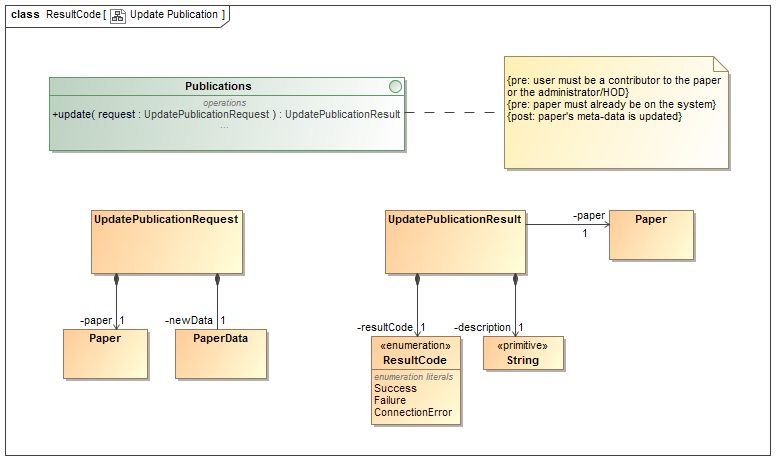
\includegraphics[width=\textwidth]{../Assignment1/5.1.6.Update.Publication.Services.Contract.png}
		\caption{Service Contract: Update Publication}
	\end{figure}
	\pagebreak
	\subsubsection{View Publication}
	
	\textbf{Description:} Allows a user/administrator/HOD to view the meta-data of a paper that lies within their permissions\\
	\textbf{Prioritisation:} Important\\
	\\
	
	\textbf{Pre-conditions}
	\begin{itemize}
		\item The user(may be the administrator or HOD) should be logged into the system.
		\item The user - if not the administrator, HOD or research leader - must be a contributor to the paper.
		\item The paper must already be in the system.
	\end{itemize}
	
	\textbf{Post-conditions}
	\begin{itemize}
		\item The paper's meta-data is displayed to the user
	\end{itemize}
	
	\begin{figure}[H]
		\centering
		%                		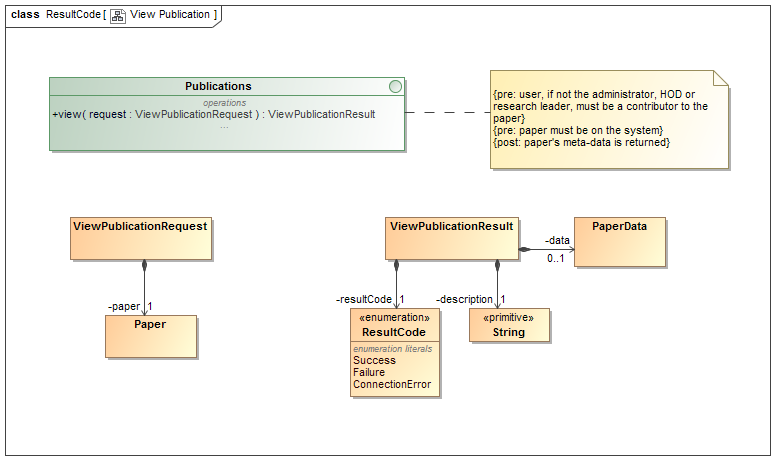
\includegraphics[width=\textwidth]{../Assignment1/5.1.7.View.Publication.Services.Contract.png}
		\caption{Service Contract: View Publication}
	\end{figure}
	
	\pagebreak
	\subsubsection{Add Publication Type}
	
	\textbf{Description:} Allows the administrator or HOD to add a publication type \\
	\textbf{Prioritisation:} Important\\
	\\
	
	
	\textbf{Pre-conditions}
	\begin{itemize}
		\item The user(must be the administrator or HOD) should be logged into the system.
		\item The publication type to add must not already be in the system.
	\end{itemize}
	
	\textbf{Post-conditions}
	\begin{itemize}
		\item The new publication type is added to the system.
	\end{itemize}
	
	
	\begin{figure}[H]
		\centering
		%            	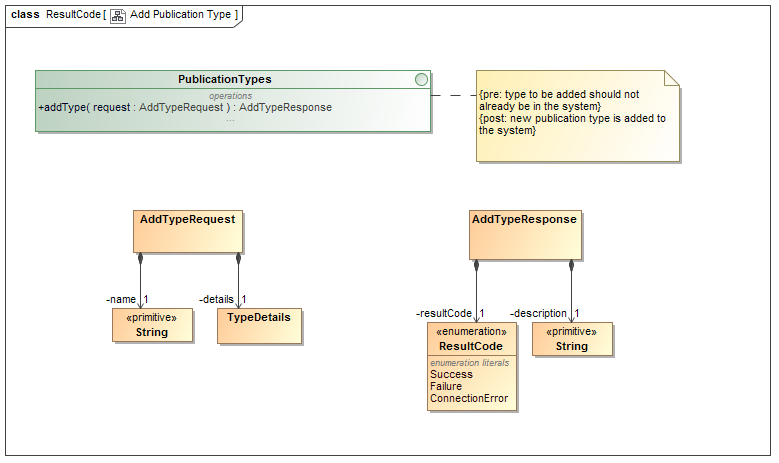
\includegraphics[width=\textwidth]{../Assignment1/5.1.8.Add.Publication.Type.Services.Contract.png}
		\caption{Service Contract: Add Publication}
	\end{figure}
	
	\pagebreak
	\subsubsection{Update Publication Type}
	
	\textbf{Description:} Allows the administrator or HOD to update a publication type's details\\
	\textbf{Prioritisation:} Important\\
	
	
	\textbf{Pre-conditions}
	\begin{itemize}
		\item The user(must be the administrator or HOD) should be logged into the system.
		\item The user - if not the administrator, HOD or research leader - must be a contributor to the paper.
		\item The publication type to be updated must already be in the system.
	\end{itemize}
	
	\textbf{Post-conditions}
	\begin{itemize}
		\item The selected publication type will be updated with the new information.
	\end{itemize}
	
	\begin{figure}[H]
		\centering
		%                	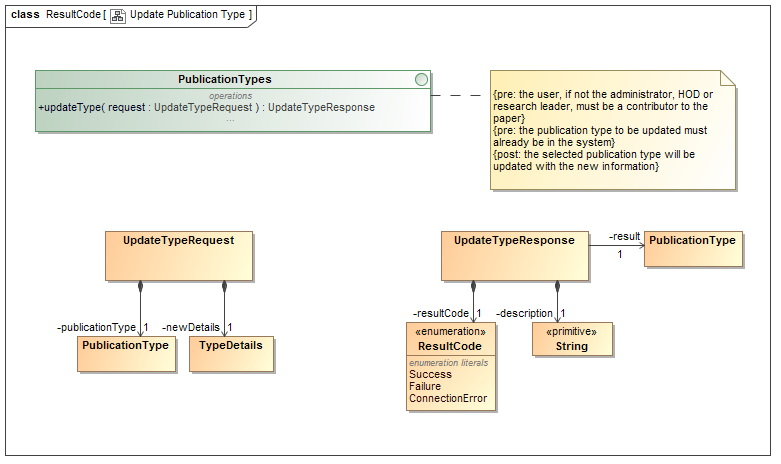
\includegraphics[width=\textwidth]{../Assignment1/5.1.9.Update.Publication.Type.Services.Contract.png}
		\caption{Service Contract: Update Publication}
	\end{figure}
	
	\pagebreak
	\subsubsection{Add Reminder}
	\textbf{Description:} Allows the user to create a reminder for the deadline of the publication.\\
	\textbf{Prioritisation:} Nice-To-Have.
	\\
	
	\textbf{Pre-conditions}
	\begin{itemize}
		\item The user(can be the HOD) should be logged into the system.
		\item The user must be a contributor to the paper.
		\item The publication must already be in the system.
	\end{itemize}
	
	\textbf{Post-conditions}
	\begin{itemize}
		\item A reminder via Mail or Calendar will be set with the selected publication and deadline.
	\end{itemize}
	
	\begin{figure}[H]
		\centering
		%                		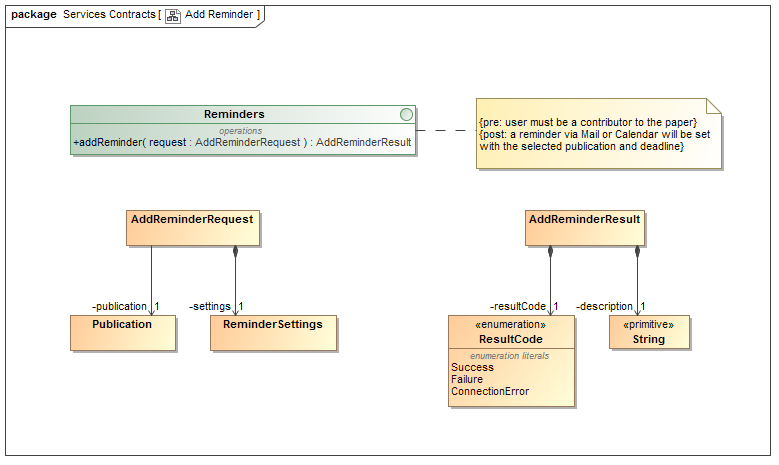
\includegraphics[width=\textwidth]{../Assignment1/5.1.10.Add.Reminder.Services.Contract.png}
		\caption{Service Contract: Add Reminder}
	\end{figure}
	
	\pagebreak
	\subsubsection{Create Research Group}
	\textbf{Description:} Allows the administrator or HOD to create a new Research Group\\
	\textbf{Prioritisation:} Critical\\
	
	\textbf{Pre-conditions}
	\begin{itemize}
		\item The user(must be the administrator or HOD) should be logged into the system.
		\item The Research Group you wish to create must not already be in the system.
	\end{itemize}
	
	\textbf{Post-conditions}
	\begin{itemize}
		\item The Research Group will be created and stored in the database.
		\item Users will be able to join the Research Group.
		\item Research Leader will be able to see all Publications made by the Research Group's members.
	\end{itemize}
	
	\begin{figure}[H]
		\centering
		%    	    		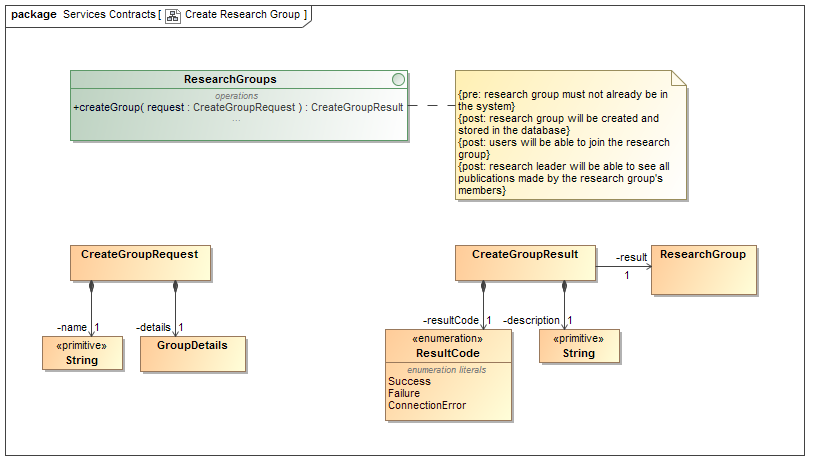
\includegraphics[width=\textwidth]{../Assignment1/5.1.11.Create.Research.Group.Services.Contract.png}
		\caption{Service Contract: Create Research Group}
	\end{figure}
	
	\pagebreak
	\subsubsection{View Research Group}
	\textbf{Description:} View the details of a Research Group \\
	\textbf{Prioritisation:} Nice-To-Have\\
	
	\textbf{Pre-conditions}
	\begin{itemize}
		\item The user(must be the administrator or HOD) should be logged into the system.
		\item The Research Group must already exist in the database.
	\end{itemize}
	
	\textbf{Post-conditions}
	\begin{itemize}
		\item The user will be able to view the details of the Research Group.
	\end{itemize}
	
	\begin{figure}[H]
		\centering
		%    	    		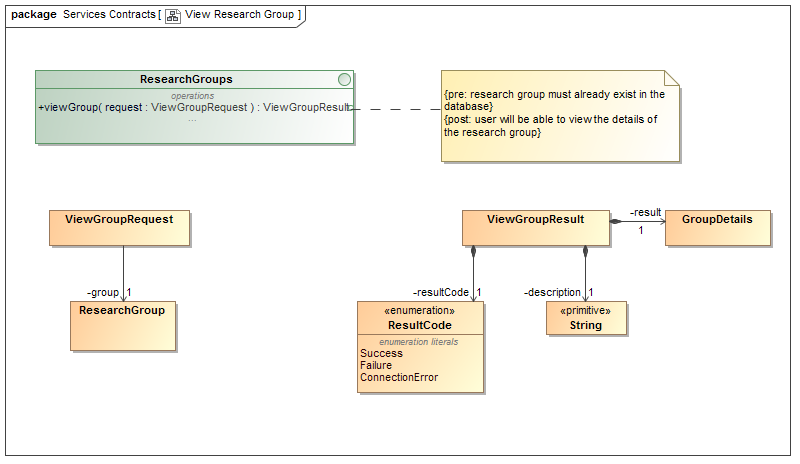
\includegraphics[width=\textwidth]{../Assignment1/5.1.12.View.Research.Group.Services.Contract.png}
		\caption{Service Contract: View Research Group}
	\end{figure}
	
	\pagebreak
	\subsubsection{Update Research Group}
	\textbf{Description:} Allows the administrator or HOD to update an existing Research Group\\
	\textbf{Prioritisation:} Important\\
	
	\textbf{Pre-conditions}
	\begin{itemize}
		\item The user(must be the administrator or HOD) should be logged into the system.
		\item The Research Group must already exist in the database.
	\end{itemize}
	
	\textbf{Post-conditions}
	\begin{itemize}
		\item The user will be able to edit and save the new information entered.
	\end{itemize}
	
	\begin{figure}[H]
		\centering
		%	    		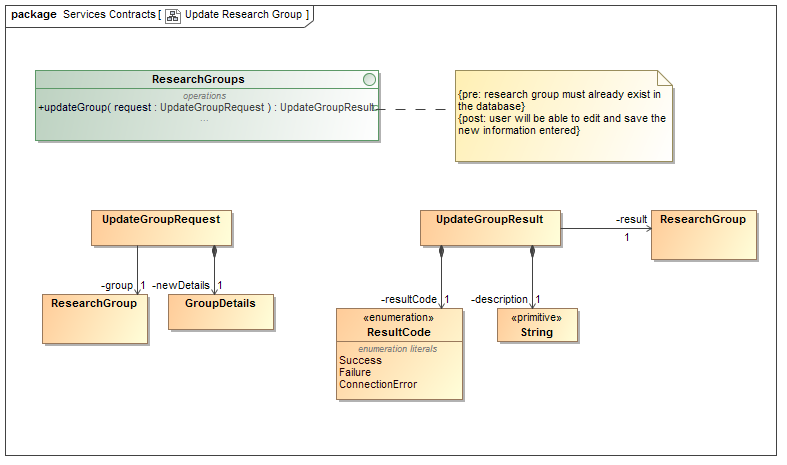
\includegraphics[width=\textwidth]{../Assignment1/5.1.13.Update.Research.Group.Services.Contract.png}
		\caption{Service Contract: Update Research Group}
	\end{figure}
	
	\pagebreak
	\subsubsection{Remove Research Group}
	\textbf{Description:} Allows the administrator or HOD to remove an existing Research Group\\
	\textbf{Prioritisation:} Important\\
	
	\textbf{Pre-conditions}
	\begin{itemize}
		\item The user(must be the administrator or HOD) should be logged into the system.
		\item The Research Group must already exist in the database.
		\item The Research Group must have no members in it and no Research Leader.
	\end{itemize}
	
	\textbf{Post-conditions}
	\begin{itemize}
		\item The user will be able to remove the Research Group from the database.
	\end{itemize}
	
	\begin{figure}[H]
		\centering
		%    	    		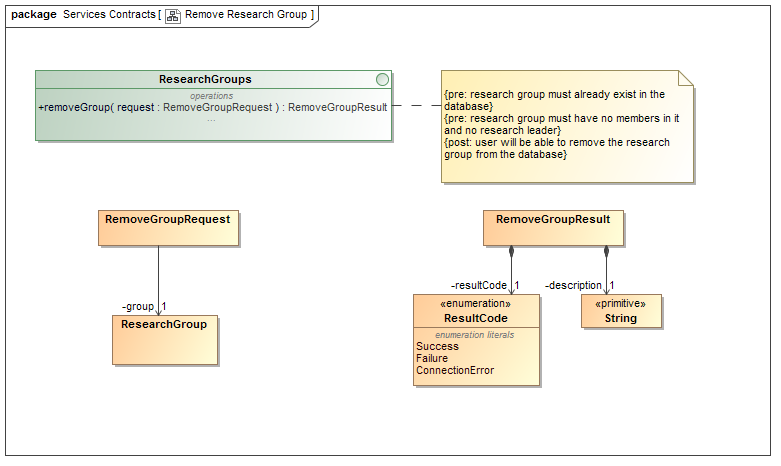
\includegraphics[width=\textwidth]{../Assignment1/5.1.14.Remove.Research.Group.Services.Contract.png}
		\caption{Service Contract: Remove Research Group}
	\end{figure}
	
	\pagebreak
	\subsubsection{Create Author}
	\textbf{Description:} Allows the user to create a new Author\\
	\textbf{Prioritisation:} Critical\\
	
	\textbf{Pre-conditions}
	\begin{itemize}
		\item The user should be logged into the system.
		\item The Author must not already exist in the database.
	\end{itemize}
	
	\textbf{Post-conditions}
	\begin{itemize}
		\item The user will be able to create a new Author and save him/her in the database.
	\end{itemize}
	
	\begin{figure}[H]
		\centering
		%    	    		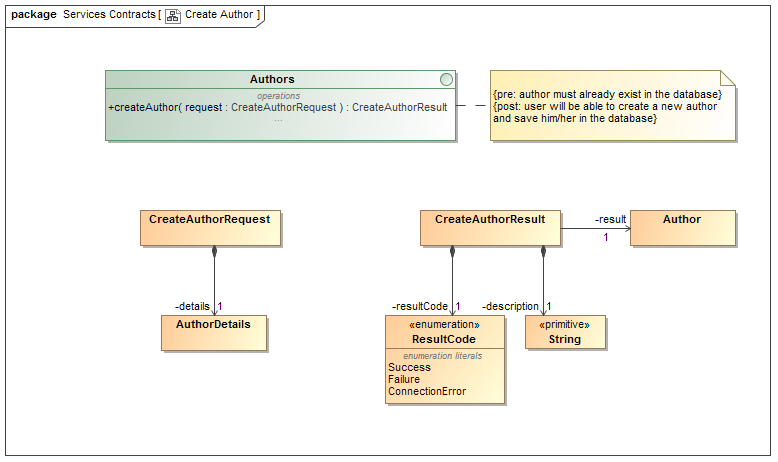
\includegraphics[width=\textwidth]{../Assignment1/5.1.15.Create.Author.Services.Contract.png}
		\caption{Service Contract: Create Author}
	\end{figure}
	
	\pagebreak
	\subsubsection{Update Author}
	\textbf{Description:} Allows the user to update an existing Author\\
	\textbf{Prioritisation:} Important\\
	
	\textbf{Pre-conditions}
	\begin{itemize}
		\item The user should be logged into the system.
		\item The Author must already exist in the database.
	\end{itemize}
	
	\textbf{Post-conditions}
	\begin{itemize}
		\item The user will be able to edit and save the new information entered.
	\end{itemize}
	\begin{figure}[H]
		\centering
		%	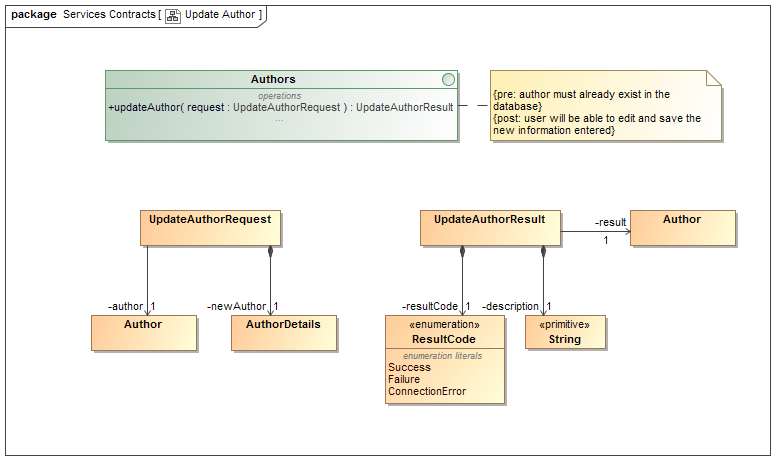
\includegraphics[width=\textwidth]{../Assignment1/5.1.16.Update.Author.Services.Contract.png}
		\caption{Service Contract: Update Author}
	\end{figure}
	
	\pagebreak
	\subsubsection{Generate Report}
	\textbf{Description:} Allows the user generate a report based on certain data\\
	\textbf{Prioritisation:} Nice to have\\
	
	\textbf{Pre-conditions}
	\begin{itemize}
		\item The user should be logged into the system.
		\item There should be existing data in the system's database
	\end{itemize}
	
	\textbf{Post-conditions}
	\begin{itemize}
		\item The system will generate a report based on certain criteria and make it visible to the user
	\end{itemize}
	\begin{figure}[H]
		\centering
		%  		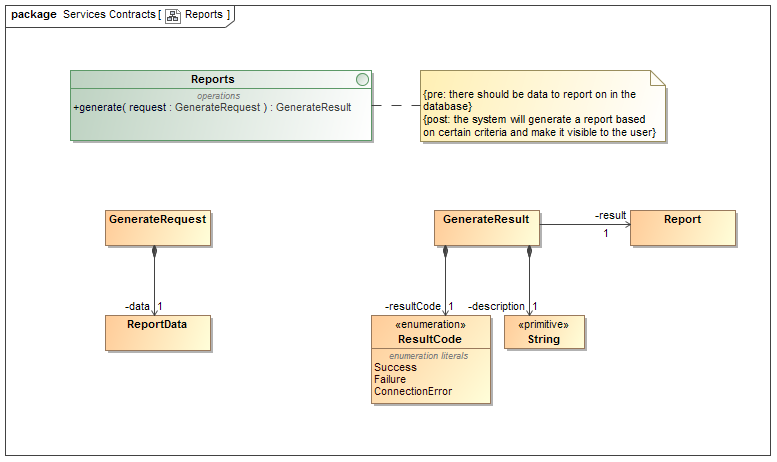
\includegraphics[width=\textwidth]{../Assignment1/5.1.17.Generate.Report.Services.Contract.png}
		\caption{Service Contract: Generate Report}
	\end{figure}
	
	\pagebreak	
	\subsection{Required Functionality}
	\subsubsection{User-Research System interaction}
	\paragraph{\textbf{Description:} The type of user indicates what privileges that user has in the Research system}
	\paragraph{\textbf{Normal-user}}
	\begin{description}
		\item[$\bullet$] A normal user may log in to the system if registered on the system.
		\item[$\bullet$] A normal user may add publications to the system.
		\item[$\bullet$] A normal user must be an author of a publication should they want to add it to the system.
		\item[$\bullet$] A normal user may add authors to a publication.
		\item[$\bullet$] A normal user may change authors in a publication.
		\item[$\bullet$] A normal user may add a publication to a conference.
		\item[$\bullet$] A normal user may only view their own publications.
	\end{description}
	\paragraph{\textbf{Head of Department}}
	\begin{description}
		\item[$\bullet$] The head of department may log in to the system.
		\item[$\bullet$] The head of department may add/edit/remove a user.
		\item[$\bullet$] The head of department may add/edit/remove an author.
		\item[$\bullet$] The head of department may add publication/edit a publication.
		\item[$\bullet$] The head of department may be an author on a publication.
		\item[$\bullet$] The head of department may add authors to a publication.
		\item[$\bullet$] The head of department may add/remove publications for conferences.
		\item[$\bullet$] The head of department may view all publications on the system.
	\end{description}
	\paragraph{\textbf{Admin}}
	\begin{description}
		\item[$\bullet$] Admin users may log in to the system.
		\item[$\bullet$] Admin users may add/remove/edit users.
		\item[$\bullet$] Admin users may add/edit publications.
		\item[$\bullet$] Admin users may not be an author to any publication on the system.
		\item[$\bullet$] Admin users may add authors to a publication.
		\item[$\bullet$] Admin users may change authors to a publication.
		\item[$\bullet$] Admin users may add/remove publications to conferences.
		\item[$\bullet$] Admin users may view all publications on the system.
	\end{description}
	\begin{figure}[H]
		%		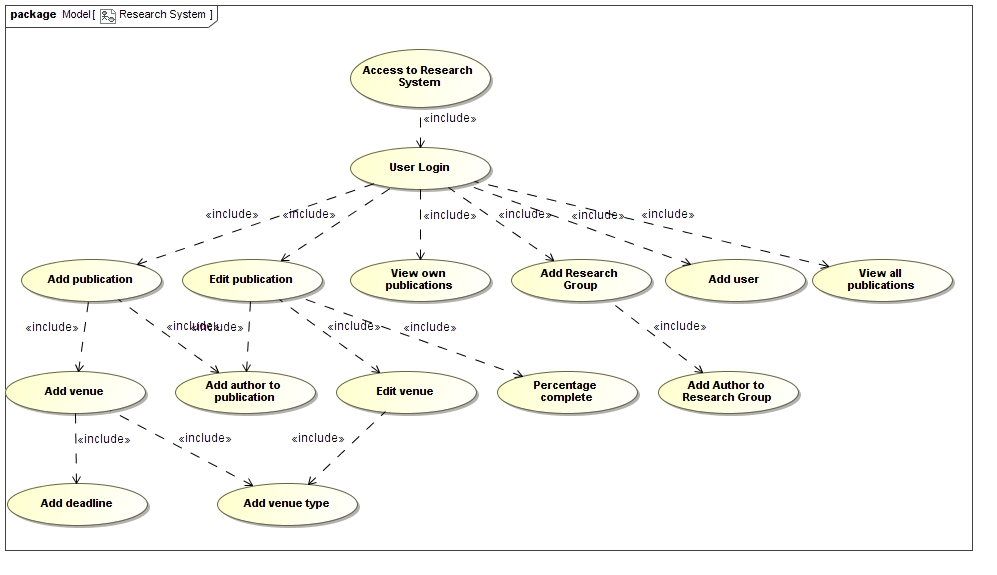
\includegraphics[width=\textwidth]{../Assignment1/Overview.jpg}
		\caption{Functional Requirements: Overview of Research System \label{overflow}}
	\end{figure}
	\begin{figure}[H]
		%		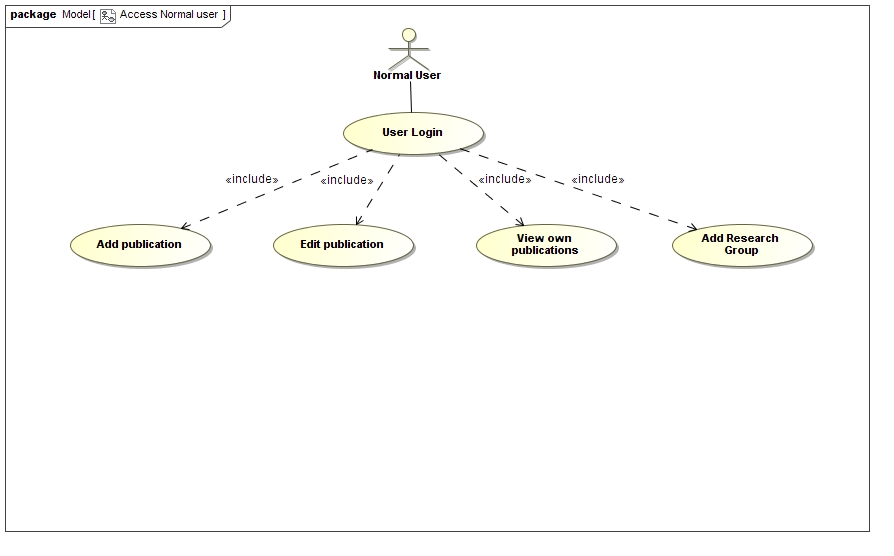
\includegraphics[width=\textwidth]{../Assignment1/AccessNormaluser.jpg}
		\caption{Functional Requirements: Normal user access privileges \label{overflow}}
	\end{figure}
	\begin{figure}[H]
		%		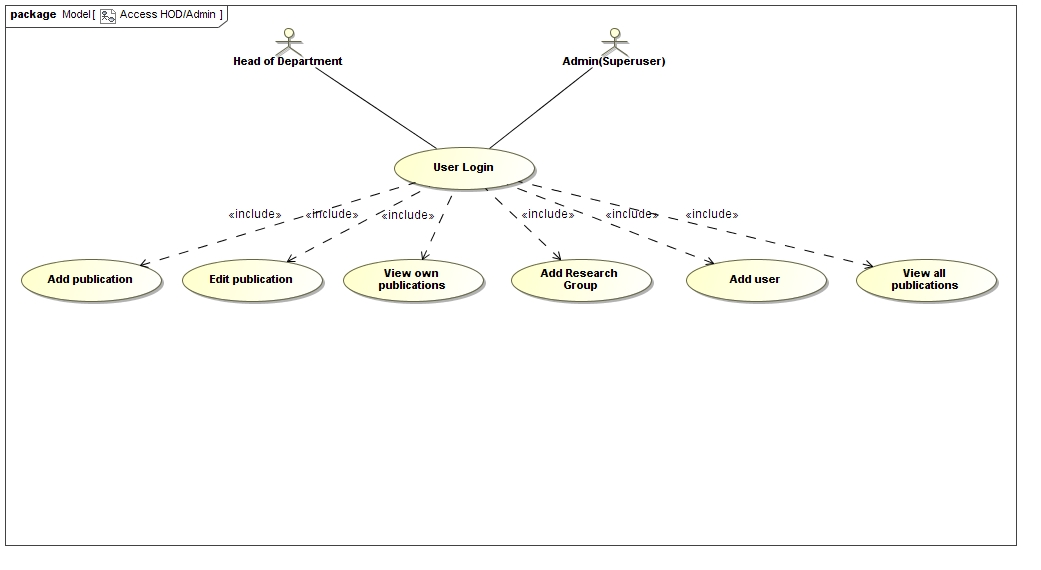
\includegraphics[width=\textwidth]{../Assignment1/AccessHODAdmin.jpg}
		\caption{Functional Requirements: Superuser(HOD and admin) access privileges \label{overflow}}
	\end{figure}
	\pagebreak
	\subsection{Process Specification}
	This section conatins UML activity diagrams that illustrate the sequences that will be followed for various use case scenarios.
	\begin{figure}[H]
		\centering
		%	    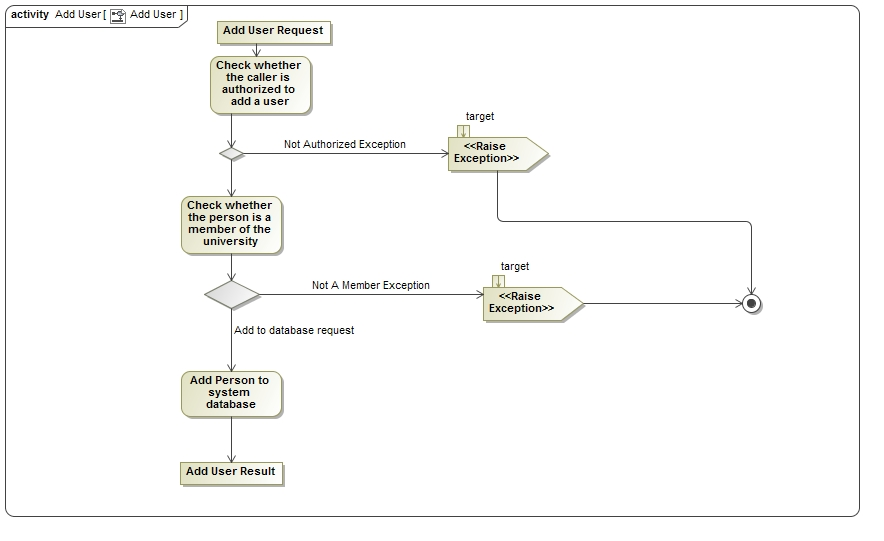
\includegraphics[width=\textwidth]{../Assignment1/AddUser.jpg}
		\caption{Process Specification: Adding A User}
	\end{figure}
	\begin{figure}[H]
		\centering
		%	    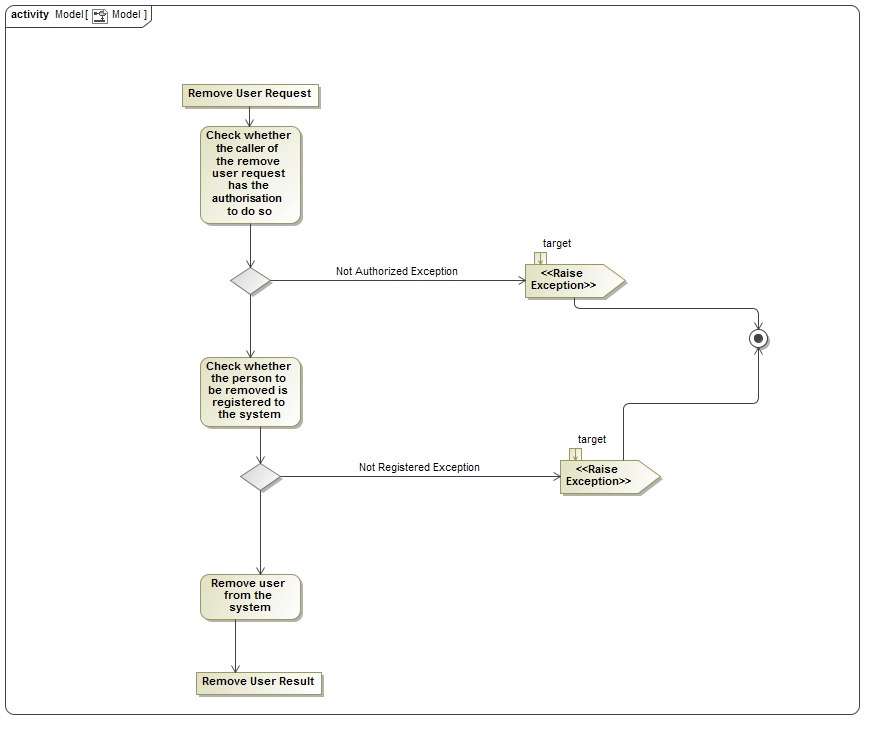
\includegraphics[width=\textwidth]{../Assignment1/removeUser.jpg}
		\caption{Process Specification: Removing A User}
	\end{figure}
	\begin{figure}[H]
		\centering
		%	    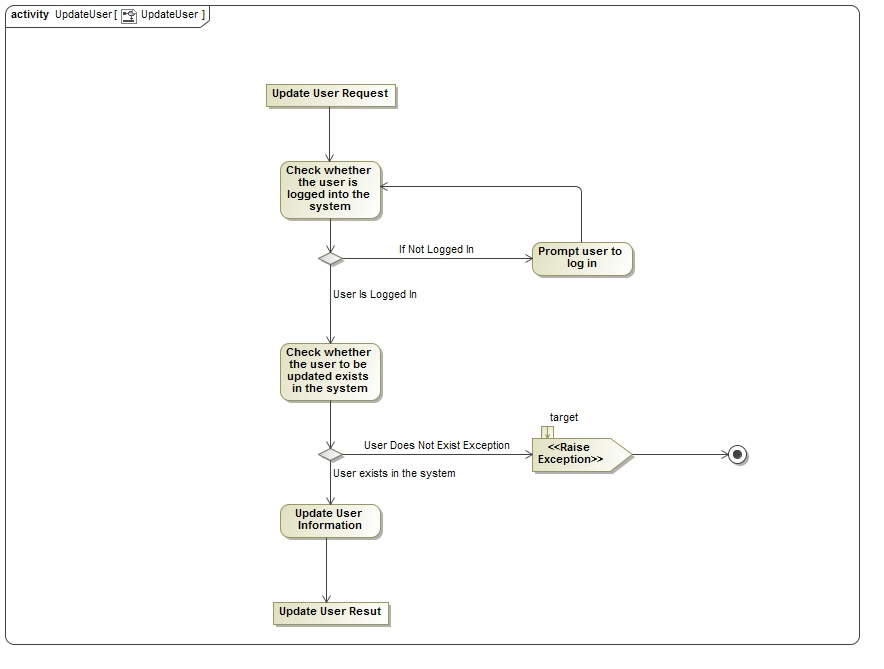
\includegraphics[width=\textwidth]{../Assignment1/UpdateUser.jpg}
		\caption{Process Specification: Update A User}
	\end{figure}
	\begin{figure}[H]
		\centering
		%	    \includegraphics[width=\textwidth]{../Assignment1/AddPublication.jpg}
		\caption{Process Specification: Adding A Publication}
	\end{figure}
	\begin{figure}[H]
		\centering
		%	    \includegraphics[width=\textwidth]{../Assignment1/UpdatePublication.jpg}
		\caption{Process Specification: Update A Publication}
	\end{figure}
	\begin{figure}[H]
		\centering
		%	    \includegraphics[width=\textwidth]{../Assignment1/ViewPublication.jpg}
		\caption{Process Specification: View A Publication}
	\end{figure}
	\subsection{Domain Model}
	\begin{figure}[H]
		%		\includegraphics[width=\textwidth]{../Assignment1/DomainModel.jpg}
		\caption{Domain Model of Research System \label{overflow}}
	\end{figure}
	\pagebreak
	\section{Open Issues}
	This section deals with issues that still need to be clarified, specified, assumed or have been discovered to include inconsistencies in the requirements, comprising of the following issues:
	\begin{description}
		\item[$\bullet$] Will a server be provided?
	\end{description}
	\begin{description}
		\item[$\bullet$] Should the HOD be a separate entity or fall within the Admin entity?
	\end{description}
	\begin{description}
		\item[$\bullet$] To where does the publication go to be reviewed?
	\end{description}
	\begin{description}
		\item[$\bullet$] Should the reminder system be via Mail or Calendar notification?
	\end{description}
	\begin{description}
		\item[$\bullet$] It is assumed that the Venue will have a deadline attached.
	\end{description}
	
\end{document}
